%%%%%%%%%%%%%%%%%%%%%%%%%%%%%%%%%%%%%%%%%%%%%%%%%%%%%%%%%%
%
% Doctoral Thesis Template @ The University of Manchester
% LaTeX Chapter Template
% Version 1 (23/07/2020)
% Joe Crone
%
% This template is based on:
% The University of Manchester, Presentation of Thesis Policy
% Research Office Graduate Education Team
% June 2017
% http://www.regulations.manchester.ac.uk/pgr-presentation-theses/
%
%%%%%%%%%%%%%%%%%%%%%%%%%%%%%%%%%%%%%%%%%%%%%%%%%%%%%%%%%%
\documentclass[../main.tex]{subfiles}
\begin{document}

% Title
%--------------------------------------------------------
\chapter{Optimisation and Characterisation of Inverse Compton Scattering Spectra}
\label{Optimisation_and_Characterisation_of_Inverse_Compton Scattering_Spectra} % to reference use \ref{ChapterTemplate}

\section{Motivation for Characterisation of ICS Sources}

Proper characterisation of inverse Compton scattering sources is necessary to quantify source performance and for reliable comparison between ICS sources. Through design and benchmarking of models used to predict ICS source performance and spectra, the ICS interactions of electron bunches and laser pulses can be better understood, which can reveal methods of improving narrowband ICS source design such as the optimisation strategies covered later in this chapter, which were motivated by the characterisation methods developed at the start of this chapter. The spectral output parameters presented in Chapter~\ref{Photon_Production_by_Inverse_Compton_Scattering}, such as flux and (average and peak) brilliance, fail to account for collimation effects, energy spread of the electron bunch and spectral bandwidth of the laser pulse. Therefore, models are required to predict the spectrum of the ICS source and quantify the affect of these parameters on the radiation spectrum available to the users of an ICS source. 

Within the first half of this chapter, an analytical approach to calculating the collimated flux produced by an ICS source is developed and compared to existing methods \cite{curatolo2017analytical} and a semi-analytical spectrum code \textsc{ICARUS}: inverse Compton scattering semi-analytical recoil-corrected ultra-relativistic spectrum code based on the model by Sun et al \cite{sun2009characterizations,sun2011theoretical}, which is corrected and expanded, is developed and benchmarked using the \textsc{ICCS3D} code \cite{krafft2016laser,ranjan2018simulation}. The characterisation methods developed here are tested through the use of three cases outlined in Section~\ref{sec:benchmarking_cases_characterisation_optimisation}, specified to cover the range of accelerators used to provide electron bunches to ICS sources, generalising the characterisation methods to any accelerator not just ERLs.

An analytical collimated flux equation has been developed in Section~\ref{sec:analytical_collimated_flux} in order to provide a quick, reliable method to predict the flux of an ICS source post-collimation with minimal assumptions. The analytical collimated flux calculation can also be used to predict the total photon yield (flux) of spectrum codes. Using this method, more accurate simulations such as those from spectrum codes can be evaluated. A wide variety of effects such as collimation, angular crossing and hourglass effects have been incorporated into this methodology, whilst the effect of energy spread of the electron bunch and spectral bandwidth of the laser pulse are notably neglected. Large-scale spectrum code simulations require computational time on the order of hours, with parallel computing whereas analytical calculations can be evaluated in sub-second timescales. Therefore, analytical collimated flux calculations are easier to apply to optimisation procedures rather than the more accurate spectral yield calculations from spectrum codes.   

The \textsc{ICARUS} spectrum code is a dedicated semi-analytical inverse Compton scattering code, which models the electron bunch--laser pulse interaction as Gaussian distributions and produces an ICS interaction spectrum
accounting for phenomena such as the recoil of the electron bunch, the emittance and divergence effects of the electron bunch and laser pulse and their energy spread and spectral bandwidth, as well as rectangular and circular collimation. However, the \textsc{ICARUS} spectrum code is limited to linear ICS interactions ($a_{0} \ll 1$) and head-on interactions ($\phi=0$). Methods have also been developed to calculate the collimated flux of an ICS source based upon these simulations. The \textsc{ICARUS} spectrum code is compared to two other ICS spectrum codes: Conglom\'{e}rat d'ABEL et d'Interactions Non-Lin\'{e}aires (\textsc{CAIN}) \cite{chen1995cain}, a Monte Carlo code for simulation of a broad range of electromagnetic interactions, and the Improved Codes for Compton Simulation (\textsc{ICCS3D}) \cite{krafft2016laser,ranjan2018simulation}, a semi-analytical code for simulation of ICS interactions. The comparison is detailed in Section~\ref{sec:} where spectrum simulation methods are discussed and the \textsc{ICARUS} code is benchmarked against the \textsc{ICCS3D} code.

\section{Analytical Collimated Flux}
\label{sec:analytical_collimated_flux}

In this section, the collimated flux - the total flux collected within an aperture of semi-angle $\theta_{\mathrm{col}}$ -- is derived from first principles, using the work of Berestetskii et al \cite{berestetskii1982quantum}. Unlike others in the literature \cite{curatolo2017analytical}, this method is valid for the angular crossing case ($\phi\in\mathbb{R}$) as the effect of the crossing angle is encompassed in the cross section as well as the geometric beam--beam angular crossing effect in Section~\ref{sec:geometric_luminosity_reduction}. The hourglass effect is also fully accounted for in this method, using the prescription of Miyahara \cite{miyahara2008luminosity}. The collimated flux calculation method is a semi-analytic calculation, requiring numerical integration, that is valid within the recoil regime (above $X\ll1$) but is only valid for the linear inverse Compton scattering case ($a_{0}\ll1$). The results of this derivation are benchmarked against a series of other methods including the \textsc{ICARUS} and \textsc{ICCS3D} spectrum codes, as well as the collimated flux formula by Curatolo et al \cite{curatolo2017analytical}, in Section~\ref{sec:benchmarking_of_the_characterisation_methods}.

From previous derivations in Section~\ref{sec:electron_photon_interaction_cross_section}, the scattering angle $\theta$ dependence of the cross section (for example the differential cross section with respect to $Y$ (Eq.~\ref{eq:differential_cross_section_Y_invariant})) arises due to the the dependence of the scattering angle on the Lorentz invariant quantities ($X$ and $Y$) (Eq.~\ref{eq:X_geometry},~\ref{eq:Y_geometry}) derived from Mandelstam variables in Section~\ref{sec:electron_photon_interactions}. Intrinsically, our definition of the recoil parameter $X$ (Eq.~\ref{eq:X_Mandelstam}) relates to the centre of mass $s$ Mandelstam variable before the interaction, so there is no scattering angle dependence as shown in (Eq.~\ref{eq:X_geometry}). However, as the $Y$ Lorentx invariant is dependent on $\theta$, to include it's scattering angle dependence we must examine the derivative of $Y$ with $\theta$. Inspecting (Eq.~\ref{eq:Y_geometry}), ahows $Y$ is also dependent on $E_{\gamma}$, the scattered photon energy (Eq.~\ref{eq:scattered_photon_energy}) derived in Section~\ref{sec:derivation_of_the_scattered_photon_energy}, which inherently is dependent on scattering angle. Thus, we must first expand $Y$ in terms of the scattered photon energy scattering angle dependence, which can be simplified in terms of the recoil parameter $X$ (Eq.~\ref{eq:X_geometry}),
\begin{equation}
Y = \frac{2\gamma E_{L}\left(1+\beta\cos\phi\right)\left(1-\beta\cos\theta\right)}{m_{e}c^{2}\left\{1-\beta\cos\theta+\left[1+\cos\left(\phi+\theta\right)\right]E_{L}/E_{e}\right\}} = \frac{X\left(1-\beta\cos\theta\right)}{1-\beta\cos\theta+\left[1+\cos\left(\phi+\theta\right)\right]E_{L}/E_{e}}.
\label{eq:Y_geometry_expanded}
\end{equation}
To find the scattering angle dependence of the cross section the derivative of $Y$ with respect to $\theta$ is required. The derivative of our expanded $Y$ Lorentz invariant (Eq.~\ref{eq:Y_geometry_expanded}) is best found using the quotient rule and the full derivative of $Y$ by $\theta$ is therefore
\begin{equation}
\frac{dY}{d\theta} = \frac{X\beta\sin\theta\left\{1-\beta\cos\theta+\left[1+\cos\left(\phi+\theta\right)\right]E_{L}/E_{e}\right\}-X\left(1-\beta\cos\theta\right)\left[\beta\sin\theta-\sin\left(\phi+\theta\right)E_{L}/E_{e}\right]}{\left\{1-\beta\cos\theta+\left[1+\cos\left(\phi+\theta\right)\right]E_{L}/E_{e}\right\}^{2}}.
\label{eq:dY_dtheta}
\end{equation}

Following the description of the interaction in Section~\ref{sec:electron_photon_interaction_cross_section}, and the subsequent derivation the differential cross section in with respect to the $Y$ Lorentz invariant in (Eq.~\ref{eq:differential_cross_section_Y_invariant}) is given by 
\begin{equation*}
\frac{d\sigma}{dY} = \frac{8\pi r_{e}^{2}}{X^{2}}\left\{\left[\left(\frac{1}{X}-\frac{1}{Y}\right)^{2}+\frac{1}{X}-\frac{1}{Y}\right]+\frac{1}{4}\left(\frac{X}{Y}+\frac{Y}{X}\right)\right\}.
\end{equation*}
To recap the derivation of (Eq.~\ref{eq:differential_cross_section_Y_invariant}) in Section~\ref{sec:electron_photon_interaction_cross_section}, we assume ambivalence over the polarisation states of the scattered photons in the double differential cross section (Eq.~\ref{eq:polarisation_differential_cross_section}) -- no single polarisation state or direction is selected -- yielding (Eq.~\ref{eq:double_differential_cross_section}), with dependence on the incident photon polarisation state. As all photons produced from any azimuthal scattering angle are collected, we integrate over the full range and the differential cross section with respect to $Y$ becomes of the form given in (Eq.~\ref{eq:differential_cross_section_Y_invariant}). Integration over the azimuthal scattering angle removes the incident photon polarisation dependence, therefore the differential cross section (Eq.~\ref{eq:differential_cross_section_Y_invariant}), and consequently the collimated flux, become independent of initial and scattered photon polarisations.

The dependence of the cross section $\sigma$ on the scattering angle $\theta$ is then given by the chain rule
\begin{equation}
\frac{d\sigma}{d\theta} = \frac{d\sigma}{dY}\frac{dY}{d\theta}.
\label{eq:cross_section_chain_rule}
\end{equation}
Therefore, the cross section for a collimation angle $\theta_{\mathrm{col}}$ becomes
\begin{equation}
\sigma\left(\theta_{\mathrm{col}}\right) = \int_{0}^{\theta_{\mathrm{col}}}\frac{d\sigma}{dY}\frac{dY}{d\theta}d\theta,
\label{eq:cross_section_integral}
\end{equation} 
where $d\sigma/dY$ is given by (Eq.~\ref{eq:differential_cross_section_Y_invariant}) and $dY/d\theta$ is given by (Eq.~\ref{eq:dY_dtheta}). The derivation of the recoil parameter (Eq.~\ref{eq:X_geometry}) accounts for the crossing angle between the incident photon and the incident electron, therefore this cross section is fully generalised for any interaction geometry.

Using the result derived in Section~\ref{sec:luminosity_and_flux}, the collimated flux is given by a modified form of the flux equation (Eq.~\ref{eq:headon_flux}), where the cross section (Eq.~\ref{eq:full_scattering_angle_cross_section_integral}) is replaced by the scattering angle dependent cross section (Eq.~\ref{eq:cross_section_integral}). The geometric luminosity angular crossing and the  hourglass effect, as explained in Section~\ref{sec:geometric_luminosity_reduction}, are taken into account using the prescription of Miyahara (Eq.~\ref{eq:miyahara_combined_reduction}) which completely generalises the collimated flux for any electron bunch--laser pulse interaction geometry. Similarly to  the uncollimated flux (Eq.~\ref{eq:flux_angular_crossing_hourglass}), the collimated flux becomes
\begin{equation}
\mathcal{F}_{\mathrm{col}} = \sigma\left(\theta_{\mathrm{col}}\right) R_{ACHG}\mathcal{L}_{\mathrm{HEAD-ON}}f.
\label{eq:collimated_flux}
\end{equation}

It is inherent in (Eq.~\ref{eq:collimated_flux}) that the interaction occurs from a point source -- the transverse and longitudinal positions of the electrons within the bunch are neglected. However, as explained in Section~\ref{sec:source_size_divergence}, the point source approximation is valid whilst the transverse (longitudinal) source size is much smaller than the collimator aperture radius (source-to-collimator distance) -- termed far-field collimation. Within (Eq.~\ref{eq:collimated_flux}) the effect of the energy spread of the bunch, the laser pulse energy spread (spectral bandwidth) and partially, via the point source approximation, the effect of the emittance (spatial extent) of the bunch are neglected. The codes \textsc{ICARUS} and \textsc{ICCS3D} \cite{krafft2016laser,ranjan2018simulation} properly take into account the energy spread factors but the emission position problem is only solved in Monte Carlo codes such as \texsc{CAIN} \cite{chen1995cain}. However, this effect is expected to be small as most ICS sources use far-field collimation.

\section{Development of the ICARUS Spectrum code}
\label{sec:development_of_the_ICARUS_spectrum_code}

\textsc{ICARUS}: inverse Compton scattering semi-analytic recoil-corrected ultra-relativistic spectrum code, uses a modified (and corrected) version of the 2D ICS spectrum model created by Sun et al. \cite{sun2009characterizations,sun2011theoretical} to generate the spectrum of radiation produced by an ICS source. The \textsc{ICARUS} code is valid for large electron recoil ($X\sim1$) and for ICS source operating in the linear regime ($a_{0}\ll 1$). \textsc{ICARUS} calculates the number of photons produced at small energy intervals that pass through a given far-field 2D collimator aperture (circular or rectangular) for the fundamental laser mode. The produced radiation spectrum is the observable ICS spectrum at a detector placed downstream of a collimator. The model assumes that the electron bunch has a 3D Gaussian distribution, approximates the laser as a 3D Gaussian pulse and can account for both circularly and linearly polarised incident photons. However, \textsc{ICARUS} is currently only valid for the head-on ($\phi = 0$) geometry.

Using the result of Sun et al \cite{sun2009characterizations,sun2011theoretical}, the distribution of a $\gamma$-ray beam produced by a head-on collision of an electron bunch and laser pulse is given by
\begin{multline}
\frac{dN_{\gamma}}{d\Omega_{c} dE_{\gamma}} = N_{e}N_{L}\int \frac{d\sigma}{d\Omega}\delta\left(\bar{E_{\gamma}}-E_{\gamma}\right)c\left(1+\beta\right)f_{e}\left(x,y,z,x',y',p,t\right)\\ \times f_L\left(x,y,z,k,t\right)dx'~dy'~dp~dk~dV~dt,
\label{eq:central_distribution_sun}
\end{multline}
where the collimator solid angle is $d\Omega_{c} = dx_{c}dy_{c}/L^{2}$ with $x_{d}$ and $y_{d}$ the $x$ and $y$ positions at the collimator and $L$ the source-to-collimator distance, $\frac{d\sigma}{d\Omega}$ is the differential cross section of the ICS interaction, $\delta\left(\bar{E_{\gamma}}-E_{\gamma}\right)$ is a delta function which encapsulates energy conservation in the process with $\bar{E_{\gamma}}$ the maximum possible energy a $\gamma$-ray have for a scattering angle $\theta$ and $E_{\gamma}$ the actual $\gamma$-ray energy, the $c\left(1+\beta\right)$ term arises from the Doppler shifting of the radiation, $f_{e}$ and $f_{L}$ are the phase-space intensity distributions of the electron bunch (Eq.~\ref{eq:electron_gaussian_intensity_distribution}) and laser pulse (Eq.~\ref{eq:laser_gaussian_intensity_distribution}) as modelled by Gaussian distributions, $dx'$ and $dy'$ are the divergence integration variables in $x$ and $y$ respectively, $dp$ is momentum of the electron integration variable, $dk$ is the wavenumber of the laser pulse integration variable, $dV$ is the volume of the interaction integration parameter and  $dt$ is the interaction time integration variable. 

The differential cross section for a head-on collision in this model is given by
\begin{equation}
\frac{d\sigma}{d\Omega} = 8\pi r_{e}^{2}\left\{\frac{1}{4}\left[\frac{4\gamma^{2}E_{L}}{\bar{E_{\gamma}}\left(1+\gamma^{2}\theta^{2}\right)}+\frac{\bar{E_{\gamma}}\left(1+\gamma^{2}\theta^{2}\right)}{4\gamma^{2}E_{\gamma}}\right]-2\cos^{2}\left(\tau-\phi_{f}\right)\frac{\gamma^{2}\theta^{2}}{\left(1+\gamma^{2}\theta^{2}\right)^{2}}\right\}\left(\frac{\bar{E_{\gamma}}}{4\gamma E_{L}}\right)^{2},
\label{eq:sun_differential_cross_section}    
\end{equation}
where $\bar{E_{\gamma}}$ is the scattered photon energy for a particular scattering angle $\theta$ in the small angle approximation for a head-on ($\phi=0$) collision
\begin{equation}
\bar{E_{\gamma}} = \frac{4\gamma^{2}E_{L}}{1+\gamma^{2}\theta^{2}+\frac{4\gamma E_{L}}{m_{e}c^{2}}}.
\label{eq:sun_Egamma_bar}    
\end{equation}
The angular divergences of the scattered photons $x'$ and $y'$ can be expressed the projection of the scattering angle of of the produced radiation in each plane $\theta_{x}'$ and $\theta_{y}'$ ($\theta = \sqrt{\theta_{x}^{2}+\theta_{y}^{2}}$) using the relations
\begin{align}
\theta_{x}' + x' &= \frac{x_{c}-x}{L}, \nonumber \\
\theta_{y}' + y' &= \frac{y_{c}-y}{L}
\label{eq:sun_angular_divergence}    
\end{align}
which arise from the geometric constraints of a photon passing through a collimator and then impinging on a detector in far-field collimation ($L \gg \sqrt{x_{c}^{2}+y_{c}^{2}}$), where $x$ and $y$ are the positions of the scattered photon on the collimator aperture in each direction. Here the small angular divergences of the laser pulse have been neglected. The model can be simply extended for collimator misalignment, through addition of a simple error term \cite{sun2009characterizations} $x/y_{\mathrm{err}}$, where the angular divergences become
\begin{align}
\theta_{x}' + x' &= \frac{x_{c}-x-x_{\mathrm{err}}}{L}, \nonumber \\
\theta_{y}' + y' &= \frac{y_{c}-x-x_{\mathrm{err}}}{L}
\label{eq:sun_collimator_misallignment}    
\end{align}

Applying (Eq.~\ref{eq:sun_angular_divergence}) and integrating (Eq.~\ref{eq:central_distribution_sun}) with respect to $dV$, the interaction volume, and $dt$ the interaction time, whilst expanding the detector solid angle, the Gaussian intensity distributions of the electron bunch (Eq.~\ref{eq:electron_gaussian_intensity_distribution}) and laser pulse (Eq.~\ref{eq:laser_gaussian_intensity_distribution}), yields
\begin{multline}
\frac{dN_{\gamma}}{dE_{\gamma}dx_{c}dy_{c}} = \frac{N_{e}N_{L}}{\left(2\pi\right)^{3}z_{R}\sigma_{p}\sigma_{k}}\int \frac{k}{\sqrt{\zeta_{x}\zeta_{y}}\sigma_{\theta_{x}}\sigma_{\theta_{y}}}\frac{d\sigma}{d\Omega}\delta\left(\bar{E_{\gamma}}-E_{\gamma}\right)\left(1+\beta\right) \\\times\exp\left[-\frac{\left(\theta_{x}-x_{c}/L\right)^{2}}{2\sigma_{\theta_{x}}^{2}}-\frac{\left(\theta_{y}-y_{c}/L\right)^{2}}{2\sigma_{\theta_{y}}^{2}}-\frac{\left(p-p_{0}\right)^{2}}{2\sigma_{p}^{2}}-\frac{\left(k-k_{0}\right)^{2}}{2\sigma_{k}^{2}}\right]~d\theta_{x}~d\theta_{y}~dp~dk,
\label{eq:sun_volume_time_integral}    
\end{multline}
where $z_{R}$ is the Rayleigh range (Eq.~\ref{eq:rayleigh_range}), and the $\zeta_{x/y}$, $\sigma_{\theta_{x/y}}$ and $\xi_{x/y}$ parameters in each plane are given by
\begin{align}
\zeta_{x} &= 1+\frac{2k\beta_{x}\epsilon_{x}}{z_{R}}, & \sigma_{\theta_{x}} &= \sqrt{\frac{\epsilon_{x}\xi_{x}}{\beta_{x}\zeta_{x}}}, & \xi_{x} &= 1+\left(\alpha_{x}-\frac{\beta_{x}}{L}\right)^{2}+\frac{2k\beta_{x}\epsilon_{x}}{z_{R}}, \nonumber\\
\zeta_{y} &= 1+\frac{2k\beta_{y}\epsilon_{y}}{z_{R}}, & \sigma_{\theta_{y}} &= \sqrt{\frac{\epsilon_{y}\xi_{y}}{\beta_{y}\zeta_{y}}}, & \xi_{y} &= 1+\left(\alpha_{y}-\frac{\beta_{y}}{L}\right)^{2}+\frac{2k\beta_{y}\epsilon_{y}}{z_{R}}, 
\label{eq:zeta_sigmatheta_xi_parameters_sun}
\end{align}
where $p_{0}$ is the reference momentum of the electron bunch and $k_{0}$ is the centroid wavenumber of the laser pulse (the wavenumber of the fundamental harmonic). Note that there is an algebraic error in Sun et al's \cite{sun2009characterizations,sun2011theoretical} derivation; Sun et al's pre-factor states that $dN/dE\propto L^{2}$ for a source-to-collimator distance $L$. The error occurs because of a mishandling of the detector solid angle. Clearly, this should be $dN/dE\propto 1/L^{2}$, meaning there is an inverse square relationship between source-to-collimator distance and the spectral density as would be expected and this is corrected within the \textsc{ICARUS} code. 

The delta function, encompassing the energy conservation of the interaction, can be re-wrote in terms of the Lorentz factor
\begin{equation}
\delta\left(\bar{E_{\gamma}}-E_{\gamma}\right) = -\delta\left(\gamma-\bar{\gamma}\right)\frac{\left(1+\bar{\gamma}^{2}\theta^{2}+\frac{4\bar{\gamma}E_{L}}{m_{e}c^{2}}\right)^{2}}{8\bar{\gamma}E_{L}\left(1+\frac{2\bar{\gamma}E_{L}}{m_{e}c^{2}}\right)},
\label{eq:sun_electron_energy_delta_function}    
\end{equation}
where $\bar{\gamma}$ is the route of $\bar{E_{\gamma}}$ (Eq.~\ref{eq:sun_Egamma_bar}), where a head-on ($\phi=0$) interaction is assumed, as given by
\begin{equation}
\bar{\gamma} = \frac{2E_{\gamma}E_{L}}{m_{e}c^{2}\left(4E_{L}-E_{\gamma}\theta^{2}\right)}\left[1+\sqrt{1+\frac{4E_{L}-E_{\gamma}\theta^{2}}{4E_{L}^{2}E_{\gamma}/\left(m_{e}c^{2}\right)^{2}}}\right].    
\end{equation}

Substituting for $\delta\left(\bar{E_{\gamma}-E_{\gamma}}\right)$ using (Eq.~\ref{eq:sun_electron_energy_delta_function}) and simply exchanging the electron bunch momentum variable from $dp$ to $d\gamma$, (Eq.~\ref{eq:sun_volume_time_integral}) is integrated with respect to $d\gamma$ to introduce the electron bunch energy spread variation, which becomes
\begin{multline}
\frac{dN_{\gamma}}{dE_{\gamma}} = \frac{r_{e}^{2}N_{e}N_{L}}{4\pi^{3}L^{2}\hbar c z_{R}\sigma_{\gamma}\sigma_{k}}\int_{k_{\mathrm{min}}}^{k_{\mathrm{max}}}\int_{-\theta_{x,\mathrm{max}}}^{\theta_{x,\mathrm{max}}}\int_{-\theta_{y,\mathrm{max}}}^{\theta_{y,\mathrm{max}}}\int_{y_{\mathrm{min}}}^{y_{\mathrm{max}}}\int_{x_{\mathrm{min}}}^{x_{\mathrm{max}}}\frac{1}{\sqrt{\zeta_{x}\zeta_{y}}\sigma_{\theta_{x}}\sigma_{\theta_{y}}}\frac{\bar{\gamma}}{1+2\gamma E_{L}/m_{e}c^{2}} \\
\times\left\{\frac{1}{4}\left[\frac{4\bar{\gamma}^{2}E_{L}}{E_{\gamma}\left(1+\bar{\gamma}^{2}\theta^{2}\right)}+\frac{E_{\gamma}\left(1+\bar{\gamma}^{2}\theta^{2}\right)}{4\bar{\gamma}^{2}E_{L}}\right]-2\cos^{2}\left(\tau-\phi_{f}\right)\frac{\bar{\gamma}^{2}\theta^{2}}{\left(1+\bar{\gamma}^{2}\theta^{2}\right)^{2}}\right\} \\
\times\exp{\left[-\frac{\left(\theta_{x}-x_{c}/L\right)^{2}}{2\sigma_{\theta_{x}}^{2}}-\frac{\left(\theta_{y}-y_{c}/L\right)^{2}}{2\sigma_{\theta_{y}}^{2}}-\frac{\left(\gamma-\gamma_{0}\right)^{2}}{2\sigma_{\gamma}^{2}}-\frac{\left(k-k_{0}\right)^{2}}{2\sigma_{k}^{2}}\right]}dx_{c}~dy_{c}~d\theta_{y}~d\theta_{x}~dk,
\label{eq:ICARUS_equation}
\end{multline}
where the cross section has been expanded in terms of the $\bar{\gamma}$ parameter with a normalisation factor in the third term, $\gamma_{0}$ is the centroid Lorentz factor of the electron bunch, $\sigma_{\gamma} = \sigma_{e}/m_{e}c^{2}$ is the spread of the Lorentz factor of the electron bunch. Integral limits have been imposed on each of the integrations, as discussed below. 

The integral over the horizontal collimator aperture $dx_{c}$ (vertical collimator aperture $dy_{c}$) can be carried out with the limits $x_{\mathrm{min}}$ and $x_{\mathrm{max}}$ ($y_{\mathrm{min}}$ and $y_{\mathrm{max}}$), which vary dependent on the collimator shape (rectangular or circular) and based on the specified collimator dimensions. For the circular collimation case, the relationship $R\geq\sqrt{x_{c}^{2}+y_{c}^{2}}$ must be obeyed with $R$ the radius of the collimator. For example, in the horizontal $x$ plane $x_{\mathrm{min}} = -R$ and $x_{\mathrm{max}} = R$, such that the limits are equal to the radius of the collimator. However this means that in the $y$ plane, the collimator position integration limits are a function of $x_{c}$: $y_{\mathrm{min}} = -\sqrt{R^{2}-x_{c}^{2}}$ and $y_{\mathrm{max}} = \sqrt{R^{2}-x_{c}^{2}}$. For the case of a rectangular collimator these limits can be treated independently.  
Integrals over the projection of the scattering angles in each plane are carried out using the limits
\begin{align}
\theta_{x,\mathrm{max}} &= \sqrt{\frac{4E_{L}}{E_{\gamma}}-\theta_{y}^{2}}, & \theta_{x,\mathrm{min}} &= -\sqrt{\frac{4E_{L}}{E_{\gamma}}-\theta_{y}^{2}} \nonumber\\ 
\theta_{y,\mathrm{max}} &= \sqrt{\frac{4E_{L}}{E_{\gamma}}}, & \theta_{y,\mathrm{min}} &= -\sqrt{\frac{4E_{L}}{E_{\gamma}}},  
\end{align}
which constrains the angular cone the radiation is produced into to a maximum of a $1/\gamma$ cone in two dimensions -- the collimation angle typically limits $E_{\gamma}$ so that the cone is smaller than $1/\gamma$. As the limits of the $\theta_{x}$ integral are dependent on $\theta_{y}$, the order of integration is constrained and $\theta_{y}$ must be evaluated before $\theta_{x}$. The order of integration is similarly constrained for the integration over a circular collimator aperture -- $x_{c}$ must be integrated before $y_{c}$.

The wavenumber $k$ of the incident laser photon in Sun et al's model \cite{sun2009characterizations,sun2011theoretical} is integrated from $0$ to $\infty$, to reflect a summation over all possible laser harmonics. However, this is impractical in a real simulation and unnecessary for laser driven sources because the fundamental harmonic is the laser wavelength of interest and other harmonics will have a negligibly weak contribution to the spectra or be excluded completely due to re-circulation in a Fabry-Perot optical cavity. Therefore, the limit for the integration of the wavenumber of the incident laser is set to $k\pm3\sigma_{k}$, representing the 3$\sigma_{k}$ spectral bandwidth tail of the laser pulse, as the laser pulse is modelled using a Gaussian distribution.  

The polarisation term $2\cos^{2}\left(\tau-\phi_{f}\right)$ in (Eq.~\ref{eq:ICARUS_equation}) must be modified as the azimuthal scattering angle $\phi_{f}$ is not explicitly integrated, instead the azimuthal scattering angle dependence is incorporated into the integration of the projection of the scattering angles ($\theta_{x}$ and $\theta_{y}$) in each plane. Therefore, the azimuthal scattering angle $\phi_{f}$ in (Eq.~\ref{eq:ICARUS_equation}) is replaced by $\phi_{f} = \cos^{-1}\left(\theta_{x}/\theta\right)$. The $x$ plane projection of the scattering angle $\theta_{x}$ is selected over the $y$ plane due to order of integration constraints. However, when integrated over the full azimuthal scattering angle ($0 \leq \phi_{f} \leq 2\pi$) -- which occurs during the spectrum code simulation -- the polarisation term is negligible as expected.

The \textsc{ICARUS} spectrum code functions as a \textsc{Mathematica} script with pre-input of ICS source parameters (electron bunch and laser pulse parameters), often from the optimisations later in this chapter, and post-processing which produces plots of spectra from the developed model and calculates the spectral yield (collimated flux) from the produced spectrum. The spectral yield (collimated flux) is calculated by 
\begin{equation}
\mathcal{F}_{\mathrm{col}} = R_{AC}f\mathcal{F}^{\mathrm{spec}}_{\mathrm{col}}    
\label{eq:spectral_yield}
\end{equation}
where $R_{AC}$ is the crossing angle luminosity reduction factor (Eq.~\ref{eq:angular_crossing_factor}), used to adjust the head-on spectrum flux for the crossing angle of the interaction as \textsc{ICARUS} only simulates head-on interactions, $f$ is the repetition rate of interactions of the source, included because the \textsc{ICARUS} simulation only simulates a single electron bunch--laser pulse interaction and $\mathcal{F}^{\mathrm{spec}}_{\mathrm{col}}$ is the spectral yield (collimated flux) of a single electron bunch--laser pulse interaction -- the area under the \textsc{ICARUS} spectrum. The spectral yield can be applied more generally to calculate the collimated flux of any head-on spectrum. 

The \textsc{ICARUS} simulation evaluates (Eq.~\ref{eq:ICARUS_equation}) at a series of scattered photon energy points to determine the number of photons produced at scattered photon energy intervals thereby building up a spectrum. The maximum scattered photon energy to sample for the spectrum calculation is calculated for the head-on case with $E_{e}+3\sigma_{e}$ as the electron bunch energy, however this neglects the laser pulse spectral bandwidth. The electron bunch energy has a squared dependence on scattered photon energy ($E_{\gamma}\propto\gamma^{2}$), in comparison to scattered photon energies linear relationship with laser wavelength, therefore it is a reasonable assumption to neglect the spectral bandwidth of the laser pulse unless the spectral bandwidth of the laser is large. The minimum sampled scattered photon energy is approximated as
\begin{equation}
E_{\gamma,\mathrm{min}} \approx E_{\gamma}\left[1-3\left(\frac{\Delta E_{\gamma}}{E_{\gamma}}\right)_{\mathrm{FWHM}}\right],
\label{eq:ICARUS_minimum_energy}
\end{equation}
where the Compton edge energy reduced by a factor of $3\sigma$, with sigma the full-width half-maximum bandwidth (Eq.~\ref{eq:FWHM_bandwidth}) of the ICS source being simulated. The minimum energy is generally appropriate for ICS spectra, however when the spectrum is highly dominated by strong collimation $E_{\gamma,\mathrm{min}}$ is much smaller than the scattered photon energy of the low energy tail of the spectrum. One hundred points in the scattered photon energy range are typically calculated, but the no. simulation points is determined due to the computational time and precision requirements of the user -- simulation time typically scales linearly with simulation points.  

For the complex integration involved in evaluating the central equation of \textsc{ICARUS} (Eq.~\ref{eq:ICARUS_equation}), quasi-Monte Carlo (QMC) integration methods are used alongside parallel-processing, where each node iterates an individual scattered photon energy point in the simulation. Typically 100 million QMC points are used to create a precise spectrum, though this simulation parameter can be adjusted with greater precision (more QMC points) costing greater simulation time. The Gaussian functions in (Eq.~\ref{eq:ICARUS_equation}) for the electron bunch energy spread and laser pulse energy spread pose a particular challenge for the numerical integration routines because these are highly oscillatory. 

To summarise, the model presented here has been adapted from the model by Sun et al \cite{sun2009characterizations,sun2011theoretical} through modification of the polarisation term in order to treat the azimuthal scattering angle dependence properly, revised integral limits for the wavenumber integration to limit this to the fundamental mode within reasonable $3\sigma_{k}$ spectral bandwidth tolerances and to correct the algebraic error involving the source-to-detector distance $L$, so the formula obeys the inverse square law. These modifications have allowed the \textsc{ICARUS} code to correctly take into account both circular and linear polarisation within the spectrum, properly account for the effect of the laser spectral bandwidth on the produced radiation (by limiting the calculation to the fundamental harmonic) and for the spectrum code to produce quantitative predictions of the spectral density, with the abandonment of the arbitrary units quoted by Sun et al \cite{sun2009characterizations,sun2011theoretical} for the spectra. This model has been built into a semi-analytical code in Mathematica designed to produce ICS spectra and calculate the collimated flux from a set of ICS source electron bunch and laser pulse parameters. Further work could include extending the model (Eq.~\ref{eq:ICARUS_equation}) for an angular crossing, accounting for non-Gaussian laser pulse and electron bunch distributions and generalising the model from the small angle and far-field collimation approximations it relies upon, though this is beyond the scope of this current work.

\section{Benchmarking Cases for Characterisation and Optimisation}
\label{sec:benchmarking_cases_characterisation_optimisation}

Three ICS source benchmarking cases are specified to be characteristic of one of three accelerator types that are considered as driver of ICS sources. The three test case ICS sources use the 're-circulated pulse` approach, using a Fabry-Perot optical cavity to re-circulate the laser pulse for interaction with a high repetition rate accelerator. Further details can be found in Section~\ref{sec:lasers_fabry_perot}, and the interaction scheme matches that shown in Figure~\ref{fig:2_mirror_4_mirror}. These three cases include: a high energy ERL driven $\gamma$-ray ICS source case (Case A), a precursor to the DIANA design in Chapter~\ref{DIANA_Inverse_Compton_Source_Design}, a storage ring case based on a $\gamma$-ray ICS source driven by the MAX-III storage ring  \cite{owen2013nonequilibrium} (Case B), and a low energy, high repetition rate linac based on the Old Dominion University x-ray ICS source design \cite{krafft2016laser,deitrick2017inverse,deitrick2018high} (Case C). For each case a single set of laser parameters is used, as discussed in Section~\ref{sec:opt_char_laser}, based on the cERL Fabry-Perot optical re-circulation cavity \cite{akagi2016narrow}.  Inclusion of a Fabry-Perot cavity in the case A ERL is as described for the DIANA ERL ICS design (Chapter~\ref{DIANA_Inverse_Compton_Source_Design}). A Fabry-Perot cavity can be incorporated within a straight -- as is the case for the DIANA ERL -- in a design like the MAX-III storage ring in case B, though proposal of a detailed optics scheme are beyond the scope of this work. The laser system envisioned in the ODU ICS \cite{krafft2016laser,deitrick2017inverse,deitrick2018high} could simply be replaced by this Fabry-Perot cavity as the IP is designed with sufficient space from the final focus triplet \cite{deitrick2018high}.

\subsection{Electron Bunch Parameters}

A series of three electron bunch cases have been devised to test both the characterisation and optimisation methods outlined within this chapter based on the three accelerator types of common interest for conventional accelerator ICS source development. The electron bunch parameters at the interaction point for each of these cases are shown in Table~\ref{tab:char_opt_electron_bunch_parameters}.

\begin{table}[!h]
\centering

\caption{Electron bunch parameters at the interaction point. Parameters are given for three cases: a state-of-the-art 1~\si{\giga\electronvolt} ERL -- a preliminary design of the DIANA ERL (Chapter~\ref{DIANA_Inverse_Compton_Source_Design}) -- (Case A), the MAX-III storage ring operated at 700~\si{\mega\electronvolt} \cite{sjostrom2009max,hansson2011imaging,rosborg2012electron} (Case B) and the designed ODU ICS 25~\si{\mega\electronvolt} high repetition rate linac \cite{krafft2016laser,deitrick2017inverse,deitrick2018high} (Case C).}
\vspace{3mm}
\resizebox{\columnwidth}{!}{
\begin{tabular}{lcccc}
\hline\hline
Parameter & Case A & Case B & Case C & Unit \\
\hline
Kinetic Energy, $E_{e}$ & 1000 & 700 & 25 & \si{\mega\electronvolt} \\
Repetition Rate, $f$ & 100 & 83.33 & 100 & \si{\mega\hertz} \\
Bunch Charge, $Q$ & 100 & 3000 & 10 & \si{\pico\coulomb} \\
Norm. Transverse Emittance, $\epsilon_{n,x}/\epsilon_{n,y}$ & 0.50/0.50 & 18.78/0.233 & 0.10/0.10 & \si{\milli\meter}-\si{\milli\radian} \\
Bunch Length, $\sigma_{e,z}$ & 1.00 & 27.9 & 0.38 & \si{\milli\meter} \\
Relative Energy Spread, $\Delta E_{e}/E_{e}$ & $10^{-4}$ & $6.07\times 10^{-4}$ & $3.00\times 10^{-4}$ & \\
\hline\hline
\end{tabular}}
\label{tab:char_opt_electron_bunch_parameters}
\end{table}

The three electron bunch cases in Table~\ref{tab:char_opt_electron_bunch_parameters} have electron bunch energies chosen to reflect the typical electron bunch energy regimes of x-ray ($E_{e} =$10's~\si{\mega\electronvolt}) and $\gamma$-ray ($E_{e} =$100's~\si{\mega\electronvolt}) production typical of most designed and operating ICS sources. Within the three electron bunch cases, each of the main accelerator driver options for ICS sources are represented: an ERL, storage ring and linac, therefore this should provide a fair overview of the applicability of the developed methods (characterisation and simulation) to a wide range of ICS source designs. The three accelerator cases in Table~\ref{tab:char_opt_electron_bunch_parameters} provide a large range in electron bunch energy (25--1000~\si{\mega\electronvolt}) as well as a large variation in bunch charge (10~\si{\pico\coulomb}--3~\si{\nano\coulomb}), tranverse normalised emittance (0.1--18.78~\si{\milli\meter}-\si{\milli\radian}) and bunch length (0.38--26.7~\si{\milli\meter}) which should be suitable for evaluating the optimisation and characterisation methods and determining their efficacy in modelling a range of ICS sources. Each of these sources has a high $\sim100$~\si{\mega\hertz} repetition rate which means they are suitable for design of high flux ICS sources using the `re-circulated pulse' approach utilising Fabry-Perot cavities, as detailed in Section~\ref{sec:lasers_fabry_perot}. The characterisation and optimisation methods are designed toward the `re-circulated pulse' approach explained in Section~\ref{sec:lasers_fabry_perot}, but can also be applied generally to any linear ($a_{0}\ll 1$) ICS source. 

Case A electron bunch parameters are typical of a world leading 1~\si{\giga\electronvolt} 3-turn energy recovery linac, which are closely related to the conceptual DIANA ERL and ICS source that is presented in Chapter~\ref{DIANA_Inverse_Compton_Source_Design}. The DIANA ERL design is based upon the design of several world-leading \si{\giga\electronvolt} ERL designs, such as the ERL based EUV-FEL design by ASML \cite{akkermans2017compact}, the PERLE energy recovery linac \cite{angal2018perle} and the ER@CEBAF ERL project \cite{meot2016er,bogacz2016er}. A full justification for the case A electron bunch parameters is near-identical to the justification of the DIANA ICS source parameters, as explained in Chapter~\ref{DIANA_Inverse_Compton_Source_Design} and consequently not repeated here.       

The electron beam parameters of case B are based upon the electron bunch parameters of the MAX-III storage ring synchrotron light source \cite{sjostrom2009max,hansson2011imaging,rosborg2012electron}. Whilst the existing accelerator does not have an ICS interaction point, a set of focusing optics and a Fabry-Perot cavity could be introduced into one of the straight sections in the 36~\si{\metre} circumference for an ICS source. Operation of MAX-III as an ICS source has been suggested by Owen et al \cite{owen2013nonequilibrium}; many other synchrotron light sources have been used as an ICS source such as HI$\gamma$S at the Duke University storage ring \cite{weller2009research}, NewSUBARU \cite{utsunomiya2015gamma} and a similar design to a MAX-III ICS source has been proposed by Pan et al \cite{pan2019design}. Whilst a range of configurations are possible for MAX-III \cite{sjostrom2009max}, including variations in operational mode such as non-equilibrium operation \cite{owen2012modular}, the parameters for case B are based on Sj\"{o}strom et al \cite{sjostrom2009max} using emittance measurements by Hansson et al \cite{hansson2011imaging} because these parameters are most typical of existing storage ring based $\gamma$-ray ICS sources such as NewSUBARU \cite{utsunomiya2015gamma} and HI$\gamma$S \cite{weller2009research}. Notably the 83.33~\si{\mega\hertz} repetition rate is lower for the case B parameters than the 100~\si{\mega\hertz} repetition rate of case A and C \cite{sjostrom2009max,rosborg2012electron}. At a current of 250~\si{\milli\amperes}, with a 36~\si{\meter} circumference and repetition rate of 83.33~\si{\mega\hertz} \cite{sjostrom2009max,rosborg2012electron} there are a total of 10 bunches with a 3~\si{\nano\coulomb} bunch charge .

Case C is based upon the design of the ODU compact linac \cite{krafft2016laser,deitrick2017inverse,deitrick2018high}, which is designed for use as a compact x-ray ICS source. The ODU ICS source is a high repetition rate ($f = 100$~\si{\mega\hertz}) linac, therefore is comparable to the ERL and storage ring ICS approaches included here and could utilise a high average power Fabry-Perot cavity for the production of x-rays. The design study for this linac is completed with start-to-end simulations and therefore beam parameters are comprehensively presented \cite{deitrick2017inverse,deitrick2018high}, which are used in this case. Small emittance and energy spread parameters of the ODU linac are attractive for development of a narrowband ICS source, hence the ODU ICS souce design is suitable for inclusion within this study.  

\subsection{Laser Pulse Parameters}

The laser parameters for the test case ICS sources, based on the electron bunch parameters in Table~\ref{tab:char_opt_electron_bunch_parameters}, are kept constant with the exception of an adjusted repetition rate for the MAX-III case B parameters where the repetition rate is reduced to 83.33~\si{\mega\hertz}. Constant laser pulse parameters for each case, shown in Table~\ref{tab:char_opt_laser_pulse_parameters}, mean the effect of the electron bunch on the ICS spectrum and optimisation is observable. The laser parameters are based upon an Nd:YAG laser ($\lambda = 1064$~\si{\nano\meter}) re-circulated in a 4-mirror Fabry-Perot optical cavity based on the cERL ICS demonstration at KEK \cite{akagi2016narrow}. The Nd:YAG laser is selected for its reasonable incident photon energy ($E_{L}-1.17$~\si{\electronvolt}), which enables scattering of high energy x-rays and $\gamma$-rays, as well as the commercially available narrow spectral bandwidth of $\Delta E_{L}/E_{L} = 4.70\times 10^{-4}$  ($\delta\lambda = 0.5$~\si{\nano\meter}) \cite{thorlabs2021ndyag200}), which is ideal for a narrowband ICS source.

\begin{table}[!h]
\centering
\caption{Laser pulse parameters at the interaction point. Each accelerator electron bunch case in Table~\ref{tab:char_opt_electron_bunch_parameters} is assumed to interact with identical laser pulse parameters at the IP.}
\vspace{3mm}
\begin{threeparttable}
\begin{tabular}{lcc}
\hline\hline
Parameter & Quantity & Unit \\
\hline
Wavelength, $\lambda_\textrm{laser}$ & 1064 & nm\\
Photon energy, $E_\textrm{laser}$ & 1.17 & eV\\
Pulse energy  & 0.1 & \si{\milli\joule}\\
Number of photons, $N_{\textrm{laser}}$ & $5.34\times 10^{14}$\\ 
Repetition rate, $f$ & 100 (83.33)\tnote{*} & MHz\\
Spot size at the IP, $\sigma_{L}$ & 30 & \si{\micro\meter}\\
Crossing angle, $\phi$ & 5 & deg \\
Pulse length  & 10 & ps\\
Spectral Bandwidth, $\Delta E_{L}/E_{L}$ & 4.70$\times 10^{-4}$ &   \\
 % 0.5nm rms error on 1064nm
\hline\hline
\end{tabular}
\begin{tablenotes}
\item[*]{Adjusted to compensate for the lower case B (MAX-III \cite{sjostrom2009max,rosborg2012electron}) repetition rate.}
\end{tablenotes}
\end{threeparttable}
\label{tab:char_opt_laser_pulse_parameters}
\end{table}

The optical cavity envisioned to deliver these laser parameters has an average stored power of 10~\si{\kilo\watt} (Case B: 8.33~\si{\kilo\watt}), well below demonstrations at MuCLS \cite{eggl2016munich} and the state-of-the-art 670~\si{\kilo\watt} stored average power optical cavity \cite{carstens2014megawatt}. A reduced average stored power is considered here because this is the current highest average stored power ICS source demonstration on an ERL, from the cERL ICS souce \cite{akagi2016narrow}. Limitations are also imposed upon the stored power of a Fabry-Perot optical cavity due to mirror heating \cite{chaikovska2016high} and the proximity of strong magnetic fields \cite{gunther2019device}, which causes thermoelatic deformation of the cavity optical mirrors and a loss of stability. At a repetition rate of 100~\si{\mega\hertz} (83.33~\si{\mega\hertz}), the cavity path length is 3~\si{\meter} (3.6~\si{\meter})  which is tolerable for both misalignment errors \cite{zomer2009polarization} and mirror heating considerations with a single stored 0.1~\si{\milli\joule} laser pulse.  

\section{Benchmarking of the Characterisation Methods}
\label{sec:benchmarking_of_the_characterisation_methods}

\subsection{ICARUS Spectrum Code}
\label{sec:ICARUS_benchmarking}

In addition to \textsc{ICARUS}, several other codes are available to produce spectra of ICS sources, using either semi-analytical or MonteCarlo approaches. Two codes have been considered for benchmarking the \textsc{ICARUS} code: \textsc{CAIN} \cite{chen1995cain}, a MonteCarlo electromagnetic interactions code, and \textsc{ICCS3D} a semi-analytical inverse Compton scattering code. \textsc{CAIN} simulation is currently viewed as the 'standard` method of simulating ICS source spectra however, the \textsc{ICCS3D} code has demonstrated some advantages for the simulation of re-circulated ICS sources with collimation, as discussed in this section. 
% CAIN - what is it + how does it work + what effects
The \textsc{CAIN} code is a MonteCarlo electromagnetic interactions code with subroutines to limit the simulated interactions to purely inverse Compton scattering interactions. A Gaussian or uniform laser distribution is generated -- specified by a superposition of plane waves -- and interacted with an electron bunch generated from a Gaussian or uniform distribution or a distribution from fole of uniformly weighted macroparticles. A MonteCarlo event generator, as specified in the \textsc{CAIN} manual \cite{yokoya2003users}, determines whether a photon is produced and then calculates a scattered photon energy and polar and azimuthal scattering angles that correspond to the scattered photon. A full description of this process is detailed in the \textsc{CAIN} manual \cite{yokoya2003users}. \textsc{CAIN} is capable of simulating non-linear ICS interactions, unlike the \textsc{ICARUS} code in Section~\ref{sec:development_of_the_ICARUS_spectrum_code} but is also limited to head-on ($\phi=0$) interactions. The emittance divergence effects of the electron bunch are accounted for by \textsc{CAIN}, but neglected for the laser pulse. Collimation is not directly implemented within the \textsc{CAIN} code but can be implemented via post processing of the produced spectra. 

% NEED MORE -HOW DOES IT WORK? WHAT EFFECTS?
The \textsc{ICCS3D} semi-analytical spectrum code, a generalization of the \textsc{ICCS} code \cite{krafft2016laser,ranjan2018simulation}, computes scattered radiation from laser pulse--electron bunch interactions within the linear Compton regime ($a_{0}\ll 1$) and accounts for electron recoil. In \textsc{ICCS3D}, a 3D laser pulse model replaces the 1D plane wave model used in \textsc{ICCS}. This modification is implemented in a manner described in Terzi\'c et al \cite{terzic2019improving}; instead of all electrons experiencing the same laser field strength $a_{0}$, as they do for a 1D plane wave, their effective laser field strength is dependent on the electron's distance from the laser's center at the moment of scattering. \textsc{ICARUS} differs from \textsc{ICCS3D} because \textsc{ICARUS} models the interaction as a collision between a laser pulse and electron bunch whereas \textsc{ICCS3D} models the interaction as an electron radiating within the electromagnetic field of a laser pulse. To calculate anticipated spectral output, in addition to the laser parameters, \textsc{ICCS3D} can use either the parameters of the electron beam or an arbitrary electron distribution -- which could be tracked through the electron accelerator -- allowing start-to-end simulation of ICS sources. The emission spectra of a single electron is calculated using a 3D laser field model and the Klein-Nishina cross section, and the spectrum is formed by summing over the emission of each individual electron. Collimation is implemented within \textsc{ICCS3D} by limiting the possible scattered photon scattering angles through which the emission is calculated. \textsc{ICCS3D} can calculate the spectrum of an ICS interaction in an angular crossing case, with square or circular collimation and accounts for the spectral bandwidth of the laser pulse, the electron bunch energy spread as well as the emittance and divergence of the electron bunch. Like the \textsc{ICARUS} code, \textsc{ICCS3D} can produce spectra for arbitrary polarisation of the incident photons.   

A semi-analytical ICS spectrum code is advantageous to Monte Carlo based techniques such as the \textsc{CAIN} spectrum code as collimation effects aren't taken into account directly within the simulation and are instead required as part of post-simulation analysis. There is no method of imposing a collimator within \textsc{CAIN} \cite{chen1995cain}. Because \textsc{CAIN} treats the incident laser pulse as a superposition of plane waves, the effect of the spectral bandwidth of the laser pulse isn't properly accounted for. Incorporating the effect of the incident laser pulse spectral bandwidth is necessary for the ICS interaction because it can be the main contributor to the bandwidth of the resulting spectrum, as is frequently the case in the `single shot' ICS source approach (see Section~\ref{sec:lasers_fabry_perot}). Inherently, in Monte Carlo simulation rare events in nature will be as rare in the simulation, therefore statistics in situations where low scattered photon counts are expected are poor; for example in the tails of the distribution, at very narrow apertures \cite{ranjan2018simulation} and in re-circulated ICS sources where low flux interactions are conducted at high repetition rate. However, \textsc{CAIN} can model non-linear ($a_{0} \sim 1$) ICS interactions unlike \textsc{ICCS3D} and \textsc{ICARUS}, which are limited to the linear regime.  

Therefore, the \textsc{ICCS3D} code \cite{krafft2016laser,ranjan2018simulation} was selected to benchmark the \textsc{ICARUS} spectrum code as \textsc{ICCS3D} also aims to predict spectra of ICS sources in the linear regime with a similar semi-analytical approach. \textsc{ICCS3D} provides a good benchmarking standard because  \textsc{ICCS3D} code has also previously been benchmarked against the 1D model by Sun et al \cite{sun2009energy} (see Krafft et al \cite{krafft2016laser} Fig.~2--4) and the \textsc{CAIN} Monte Carlo code (see Ranjan et al\cite{ranjan2018simulation} Fig.~7). Consequently, benchmarking \textsc{ICARUS} against \textsc{ICCS3D} means we can be confident that \textsc{ICARUS} would perform reasonably against \textsc{CAIN}. Through benchmarking of \textsc{ICARUS} against \textsc{ICCS3D}, \textsc{ICCS3D} has also been improved via introduction of a new integration method to handle laser pulse durations on the order of 10's~\si{\pico\seconds} and the application of non-arbitrary units in the simulation.

\textsc{ICARUS} spectra have been produced for the three configurations of ICS source (case A, B snd C) outlined in Section~\ref{sec:benchmarking_cases_characterisation_optimisation}, as shown in Figure~\ref{fig:ICARUS_optimised_benchmarking}. The head-on ($\phi=0$) spectra in Fig.~\ref{fig:ICARUS_optimised_benchmarking} are produced using the optimised electron bunch $\beta$-functions and collimation parameters from a 0.5\% \textit{rms} bandwidth (2\% \textit{rms} bandwidth for case B) genetic algorithm optimisation (detailed in Section~\ref{sec:NRB_optimisation}), as shown in Table~\ref{tab:single_point_optimisations}, because collimation and $\beta$-functions at the IP are not defined in Table~\ref{tab:char_opt_electron_bunch_parameters}. Spectra have also been produced, courtesy of B. Terzi\'{c}, using \textsc{ICCS3D} using identical configurations for cases A, B and C as shown in Fig.~\ref{fig:ICARUS_optimised_benchmarking}.       

\begin{figure}[!h]
\centering
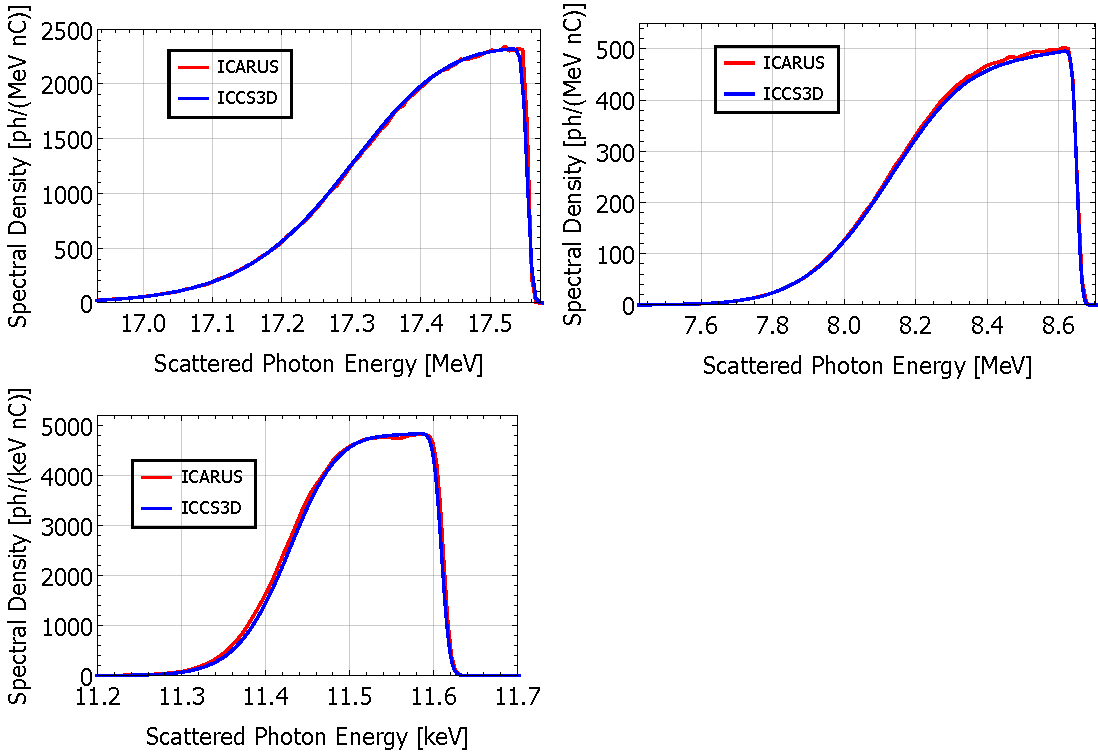
\includegraphics[width=\textwidth]{Figures/Optimisation_and_Characterisation_of_Inverse_Compton_Scattering_Sources/ICARUS_ICCS3D_cases_comparison.pdf}
\caption{Comparison of ICS head-on ($\phi=0$) single electron bunch--laser pulse interaction spectra using circular collimation for each case in Table~\ref{tab:char_opt_electron_bunch_parameters}, produced by the semi-analytical codes \textsc{ICARUS} (red) and \textsc{ICCS3D} (blue) for 0.5\% \textit{rms} bandwidth, with configuration optimised by the single point GA non-round beam optimisation  (see Section~\ref{sec:NRB_optimisation}). All \textsc{ICARUS} spectra are produced using $100\times 10^{6}$ QMC points and sampled at 100 points across the energy range. Top Left: Case A. Top Right: Case B. Bottom Left: Case C.}
\label{fig:ICARUS_optimised_benchmarking}
\end{figure}

The \textsc{ICARUS} and \textsc{ICCS3D} spectra for cases A, B and C in Fig.~\ref{fig:ICARUS_optimised_benchmarking} show good agreement. The spectra in each case produced via \textsc{ICARUS} and \textsc{ICCS3D} are near-identical in shape, with identical peak spectral density and Compton edge energies (Eq.~\ref{eq:compton_edge_energy}) -- the scattered photon energy at peak spectral density -- in both of the spectra for each case. Consequently, the spectral yield (collimated flux) is in good agreement between the two codes -- an agreement in collimated flux of $< 2\%$ is noted for each of the benchmarking cases.

Through collaboration with the \textsc{ICCS3D} \cite{krafft2016laser,ranjan2018simulation,terzic2019improving} designers and benchmarking with \textsc{ICARUS} an integration problem has been noted in \textsc{ICCS3D} where the spectrum code was producing incorrect results for long electron bunch and laser pulse lengths, which was corrected during benchmarking for the CBETA ICS source in Chapter~\ref{CBETA_Inverse_Compton_Scattering_Source_Design}.
\textsc{ICCS3D} was previously quoted in arbitrary units because it was benchmarked against the spectrum model by Sun et al \cite{sun2009characterizations}, which contained the inverse square law error described in Section~\ref{sec:development_of_the_ICARUS_spectrum_code}. Through understandin of the inverse square law error and the good agreement shown in Fig.~\ref{fig:ICARUS_optimised_benchmarking} the arbitrary units could be replaced with the proper units of the spectral density, allowing \textsc{ICARUS} and \textsc{ICCS3D} to quantitatively predict the results of ICS experiments.   

However, oscillatory behaviour or 'roughness` -- quickly varying amplitude of the spectral density -- is present in the shape of the \textsc{ICARUS} spectra because of the highly oscillatory integrals involved in the electron bunch energy spread term of (Eq.~\ref{eq:ICARUS_equation})
\begin{equation}
\frac{dN_{\gamma}}{dE_{\gamma}} &\propto \exp\left[\frac{\left(\gamma-\gamma_{0}\right)^{2}}{2\sigma_{\gamma}^{2}}\right],
\label{eq:ICARUS_electron_energy_spread_term}
\end{equation}
which causes errors in the quasi-Monte Carlo integration. The 'roughness` effect appears unphysical and, upon further investigation, seems related to the number of quasi-Monte Carlo integration points used in the simulation. 

Therefore, two simulation parameters which could affect the quality of the \textsc{ICARUS} simulation have been further investigated: the number of simulation points the model (Eq.~\ref{eq:ICARUS_equation}) is evaluated for and the number of quasi-Monte Carlo points used in the integration. Both have been investigated using case A  in Table~\ref{tab:char_opt_electron_bunch_parameters}, with collimation and $\beta$-functions at the IP specified by a 0.5\% \textit{rms} bandwidth optimisation using the non-round beam genetic algorithm method ($\theta_{\mathrm{col}}=0.066$~\si{\milli\radian}, $\beta_{x}^{*}=2.11$~\si{\meter}, $\beta_{y}^{*}=0.867$~\si{\meter}), as is used in Fig.~\ref{fig:ICARUS_optimised_benchmarking}. The investigation into the study of the number of simulation points produces \textsc{ICARUS} spectra with a range of 10--300 simulation points and a constant $5\times 10^{7}$ QMC points. Whereas the study of the number of QMC points produces \textsc{ICARUS} spectra with 100 simulation points and 10--100 million QMC points. The results of the simulation and QMC point investigations are shown in Fig.~\ref{fig:ICARUS_sim_qmc_points}

\begin{figure}[!h]
\centering
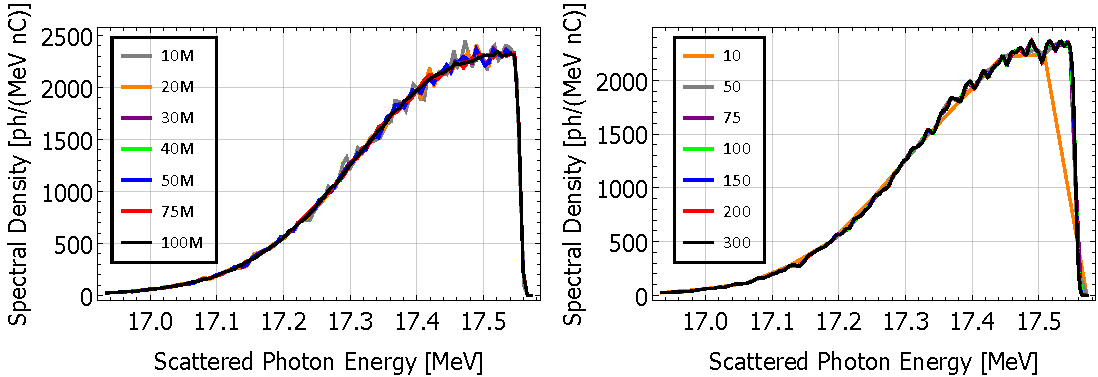
\includegraphics[width=\textwidth]{Figures/Optimisation_and_Characterisation_of_Inverse_Compton_Scattering_Sources/QMC_SIM_POINT_STUDY.pdf}
\caption{Left: A series of \textsc{ICARUS} spectra for varying number of quasi-MonteCarlo points (M=million) used within the integration routine, performed for 100 simulation points using Case A. More integration points produce a smoother spectrum -- the oscillations in the spectra are due to integration errors. Right: A series of \textsc{ICARUS} spectra for varying number of simulation points, performed with 50 million QMC points using Case A. Too few points results in a poorly defined spectra.}
\label{fig:ICARUS_sim_qmc_points}
\end{figure}

% write about all that
The study of the number of simulations points shows that the spectrum is poorly defined and hard-edged for a low number of simulation points, for example the 10 simulation points spectrum in Fig.~\ref{fig:ICARUS_sim_qmc_points}. Beyond $\sim 100$ simulation points the shape of the spectrum is not noticeably improved, therefore 100 simulation points is a reasonable number of simulation points for an \textsc{ICARUS} simulation. The simulation time increases near-linearly with increasing simulation points; with 100 simulation points the simulation time is 64~\si{\minute} and 300 simulation points requires 194~\si{\minutes}. Therefore $< 100$ simulation points only increases the time of the simulation not the quality.

In Fig.~\ref{fig:ICARUS_sim_qmc_points}, the \textsc{ICARUS} spectra are shown for varying quantities of quasi-Monte Carlo integration points; the spectral shape improves with number of quasi-Monte Carlo points utilised as the 'roughness` of the spectral shape  originating from the oscillatory integral of the electron bunch energy spread term is removed. The 'roughness` is deemed unphysical because the amplitude of the spectral density oscillations present in the case A spectrum are reduced with additional quasi-Monte Carlo integration points which increase the accuracy of the integration. However, increasing the number of QMC points used in the simulation increases the simulation time. For example, a 100 million QMC point \textsc{ICARUS} simulation increases the simulation time $\sim 12$ fold over a 10 million QMC point simulation.    

\subsection{Analytical Collimated Flux}

The analytical collimated flux (Eq.~\ref{eq:collimated_flux}) derived in Section~\ref{sec:analytical_collimated_flux} has been compared against numerous methods including the analytical formulation by Curatolo et al \cite{curatolo2017analytical} as well as the collimated flux (spectral yield) calculated from the \textsc{ICARUS} and \textsc{ICCS3D} \cite{krafft2016laser,ranjan2018simulation} spectrum codes. The collimated flux is calculated by Curatolo et al, in 'natural units` as 
\begin{equation}
\mathcal{F}_{\mathrm{col}} = 6.25\times 10^{8}\frac{E_{\mathrm{pulse}}\left(\mathrm{\si{\joule}}\right)Q\left(\si{\pico\coulomb}\right)f\left(\si{\hertz}\right)}{E_{L}\left(\si{\electronvolt}\right)\left[\sigma_{e}^{2}\left(\si{\micro\meter}\right)+\sigma_{L}^{2}\left(\si{\micro\meter}\right)\right]}\times\frac{\left(1+\sqrt[3]{X}\Psi^{2}/3\right)\Psi^{2}}{\left[1+\left(1+X/2\right)\Psi^{2}\right]\left(1+\Psi^{2}\right)},
\label{eq:curatolo_collimated_flux}
\end{equation}
where all units are consistent with those in (Eq.~\ref{eq:collimated_flux}), $\Psi-\gamma\theta_{\mathrm{col}}$ is the acceptance angle and $\sigma_{e} = \sqrt{\sigma_{x}^{2}+\sigma_{y}^{2}}$ is the \texit{rms} spot size of the electron bunch at the IP, with $\sigma_{x/y}$ the \textit{rms} spot size in each plane.

The collimated flux calculation by Curatolo et al \cite{curatolo2017analytical} (Eq.~\ref{eq:curatolo_collimated_flux}) uses the Berestetskii, Pitaevskii and Lifshitz \cite{berestetskii1982quantum} differential cross section (Eq.~\ref{eq:differential_cross_section_Y_invariant}) as in the derivation presented here in Section~\ref{sec:analytical_collimated_flux} however, an explicit derivation is not shown or referenced. Upon inspection of (Eq.~\ref{eq:curatolo_collimated_flux}), it is evident that this is only valid for a head-on ($\phi=0$) interaction and doesn't account for the  hourglass effect \cite{furman1991hourglass,miyahara2008luminosity} -- the luminosity reduction due to interaction of a diverging laser pulse and electron bunch -- outlined in Section~\ref{sec:geometric_luminosity_reduction}. Therefore, to align the Curatolo et al calculations (Eq.~\ref{eq:curatolo_collimated_flux}), the angular crossing and hourglass effect luminosity reduction factor $R_{ACHG}$ \cite{miyahara2008luminosity} (Eq.~\ref{eq:miyahara_combined_reduction}) must be introduced.  The cross section in (Eq.~\ref{eq:curatolo_collimated_flux}) appears to assume the Thomson cross section, not the recoil corrected cross section, unlike the calculation in (Eq.~\ref{eq:collimated_flux}).

The collimated flux calculation methods are compared using the benchmarking cases in Section~\ref{sec:benchmarking_cases_characterisation_optimisation} with the electron bunch parameters in Table~\ref{tab:char_opt_electron_bunch_parameters} and laser pulse parameters in Table \ref{tab:char_opt_laser_pulse_parameters}). The calculations have been conducted using the genetic algorithm single point bandwidth optimisation, as outlined in Section~\ref{sec:NRB_optimisation}, for a 0.5\% \textit{rms} bandwidth (2\% \textit{rms} bandwidth case B) which yields the values for the $\beta$-functions at the IP and collimation angle shown later in this chapter in Table~\ref{tab:single_point_optimisations}. The results of the collimated flux calculations, by each method, for each of the benchmarking cases A, B and C are shown in Table~\ref{tab:collimated_flux_calculations}

\begin{table}[!h]
\centering
\caption{\textcolor{blue}{**CAPTION TO DO**}}
\vspace{3mm}
\begin{threeparttable}
\begin{tabular}{lccc}
\hline\hline
 & \multicolumn{3}{c}{Collimated Flux (ph/\si{\second})} \\
\hline
Method & Case A & Case B & Case C \\
\hline 
Curatolo et al~\tnote{*} (Eq.~\ref{eq:curatolo_collimated_flux}) \cite{curatolo2017analytical} & $6.03 \times 10^{8}$ & $5.95\times 10^{9}$ & $7.35\times 10^{7}$ \\
Analytical (Eq.~\ref{eq:collimated_flux}) & $8.86 \times 10^{8}$ & $1.04 \times 10^{10}$ & $1.17\times 10^{8}$ \\
\textsc{ICARUS}~\tnote{$\dagger$} (Eq.~\ref{eq:spectral_yield}) & $8.76\times 10^{8}$ & $1.04\times 10^{10}$ & $1.14\times 10^{8}$ \\
\textsc{ICCS3D}~\tnote{$\dagger$} (Eq.~\ref{eq:spectral_yield}) \cite{krafft2016laser,ranjan2018simulation} & $8.75\times 10^{8}$ & $1.02\times 10^{10}$ & $1.16\times 10^{8}$  \\
\hline\hline
\end{tabular}
\begin{tablenotes}
\item[*]{The Curatolo et al collimated flux (Eq.~\ref{eq:curatolo_collimated_flux}) has been multiplied by the combined angular crossing and hourglass effect luminosity reduction factor (Eq.~\ref{eq:miyahara_combined_reduction}) for comparison with other collimated flux calculations.}
\item[$\dagger$]{The \textsc{ICARUS} and \textsc{ICCS3D} spectra used in the calculation of the collimated flux (spectral yield) are shown in Fig.~\ref{fig:ICARUS_optimised_benchmarking}.}
\end{tablenotes}
\end{threeparttable}
\label{tab:collimated_flux_calculations}
\end{table}

The collimated flux calculations in Table~\ref{tab:collimated_flux_calculations} show good agreement between the spectrum code calculations, as \textsc{ICARUS} and \textsc{ICCS3D} agree to within $< 2\%$ in all cases. Good agreement was shown qualitatively between these two codes in Fig.~\ref{fig:ICARUS_optimised_benchmarking}, therefore good quantitative agreement was expected. Between the \textsc{ICARUS} code and the analytical collimated flux calculation (Eq.~\ref{eq:collimated_flux}), a maximum discrepancy of 1.14\% is observed. Percentage scale discrepancies between these two calculations can be expected because the analytical calculation neglects the energy spread of the electron bunch and the spectral bandwidth of the laser pulse and the \textsc{ICARUS} code is not exact because of oscillatory integration errors, as discussed in Section~\ref{sec:ICARUS_benchmarking}. 

However, the collimated flux calculation by Curatolo et al \cite{curatolo2017analytical} (Eq.~\ref{eq:curatolo_collimated_flux}) shows large discrepancies from both the analytical collimated flux derived in Section~\ref{sec:analytical_collimated_flux} and the spectrum codes. Table~\ref{tab:collimated_flux_calculations} shows the Curatolo et al collimated flux (Eq.~\ref{eq:curatolo_collimated_flux}) is consistently reduced with reference to the analytical (Eq.~\ref{eq:collimated_flux}) and spectrum code collimated flux, which is also observed in Fig.~\ref{fig:curatolo_collimated_flux_comparison}. For example, in Table~\ref{tab:collimated_flux_calculations}, a factor $\sim 1.75$ reduction in collimated flux is observed between (Eq.~\ref{eq:collimated_flux}) and (Eq.~\ref{eq:curatolo_collimated_flux}) for case B. The discrepancy must originate in the angular term of (Eq.~\ref{eq:curatolo_collimated_flux})
\begin{equation*}
\mathcal{F}_{\mathrm{col}}\propto\frac{\left(1+\sqrt[3]{X}\Psi^{2}/3\right)\Psi^{2}}{\left[1+\left(1+X/2\right)\Psi^{2}\right]\left(1+\Psi^{2}\right)}    
\end{equation*}
because the head-on luminosity is equivalent in both equations, the geometric luminosity reduction is applied identically and the cross section variation of Case A (the maximum electron bunch energy case, $E_{e}=1$~\si{\giga\electronvolt}) is small -- a 1.2\% reduction in the ICS cross section (Eq.~\ref{eq:compton_cross_section_classical_limit}). The cross section variation with electron energy is illustrated in Fig.~\ref{fig:cross_section_electron_energy}. However, the origin of the discrepancy in the angular term of the Curatolo et al \cite{curatolo2017analytical} calculation (Eq.~\ref{eq:curatolo_collimated_flux}) remains unknown because no adequate derivation is shown within the literature.   

To further investigate the angular dependency of the collimated flux calculations the collimated flux, via the two analytical methods (Eqs.~\ref{eq:collimated_flux}, \ref{eq:curatolo_collimated_flux}) and the \textsc{ICARUS} spectrum code, has been calculated as a function of the acceptance angle in Fig.~\ref{fig:curatolo_collimated_flux_comparison}. 
% mention where the parameters are from
  
\begin{figure}[!h]
\centering
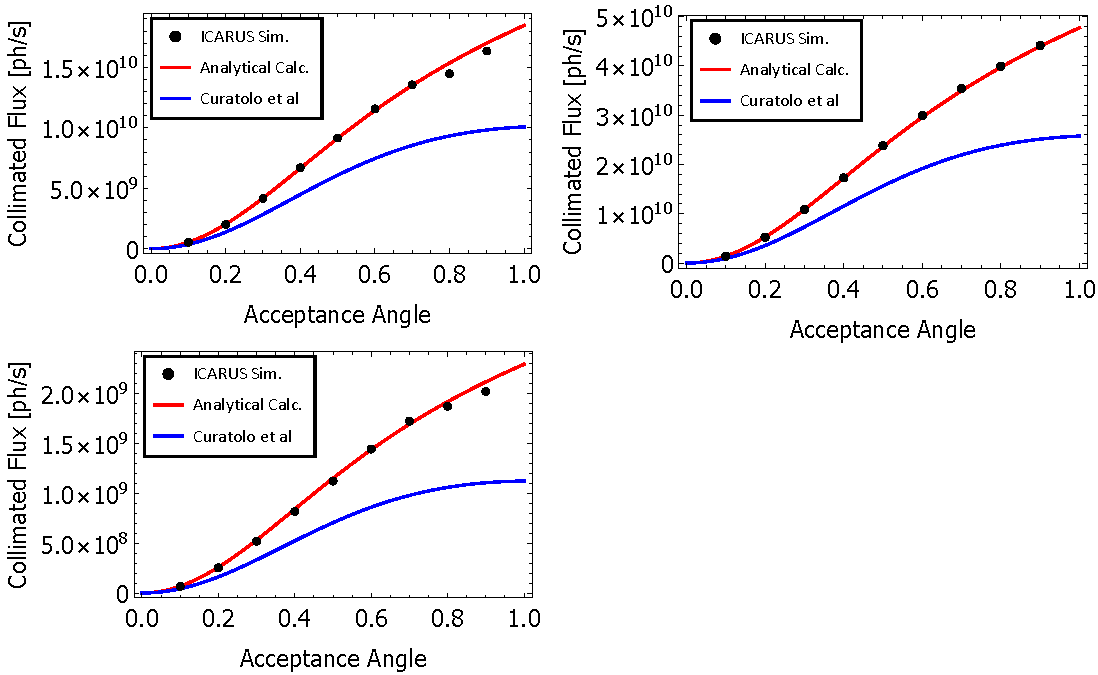
\includegraphics[width=\textwidth]{Figures/Optimisation_and_Characterisation_of_Inverse_Compton_Scattering_Sources/Fcol_PSI_Cases_Curatolo_Analytical_ICARUS.pdf}
\caption{\textcolor{blue}{**re-write caption**}Comparison of the derived analytical calculation in this work (Eq.~\ref{eq:collimated_flux}) (blue) with the Curatolo et al \cite{curatolo2017analytical} calculation (Eq.~\ref{eq:curatolo_collimated_flux}) (red) within an acceptance angle $0 \geq \Psi \geq 1$ (a $1/\gamma$ cone). Electron bunch and laser pulse spot sizes are matched ($\sigma_{e}=\sigma_{L}=30$~\si{\micro\meter}). Left: (Eq.~\ref{eq:collimated_flux}) includes hourglass effect ($R_{ACHG}\neq 1$). Right: (Eq.~\ref{eq:collimated_flux}) neglects the angular crossing and hourglass effect ($R_{ACHG} = 1$). Top: Case A. Middle: Case B. Bottom: Case C. \textcolor{blue}{**ADD THE ICARUS RUNS TO THESE PLOTS, LIKE BALSA HAS WITH THE BW COMPARISON**}}
\label{fig:curatolo_collimated_flux_comparison}
\end{figure}

\textcolor{blue}{**WRITE ABOUT THE COL FLUX ANGLE PLOTS**}

The analytical calculation (Eq.~\ref{eq:collimated_flux}) is proficient at calculating the yield of ICS spectrum codes within energy spread and spectral bandwidth tolerances and consequently is a valid alternative to spectrum code collimated flux calculations. The analytical collimated flux calculation is advantageous in terms of simulation time, as the collimated flux is calculated analytically on a sub-second timescale whereas the spectrum codes at 100 million QMC points and 100 simulation points require hours to run. Consequently, the analytical collimated flux is a useful calculation method for computing the many collimated flux values required in the optimisations detailed in the rest of this chapter.   

\section{Motivation for Narrowband Optimisation of ICS Sources}
\label{sec:motivation_optimisation}

Currently, many ICS sources \cite{deitrick2017inverse,deitrick2018high} \textcolor{blue}{**NEED MORE**} are designed with regard to producing the maximum uncollimated flux from the ICS interaction. However, within design of an inverse Compton scattering source for light source experimentation there are two objectives: to produce a large quantity of photons and to minimise the energy spread i.e bandwidth of the scattered radiation towards a monochromatic source. The former, a high flux of photons, is desirable because a high flux speeds up data acquisition times and can improve the signal-to-noise ratio of measurements and the later is advantageous due to the ability to target only a certain process, for example a specific resonance in $^{235}\mathrm{U}$ in a nuclear resonance fluorescence investigation. Users typically require a compromise on bandwidth and flux to have enough precision to investigate a specific phenomena whilst needing to make measurements on a reasonable timescale, with adequate statistics. Therefore, within the following optimisations we aim to maximise the collimated flux (Eq.~\ref{eq:collimated_flux}) whilst minimising, or limiting to some user specified value, the \textit{rms} bandwidth (Eq.~\ref{eq:RMS_bandwidth}) of the source. All optimisations are performed with the assumption of a circular collimator as the focus of this study is on narrow bandwidth and the studies within Section~\ref{sec:benchmarking_of_the_ICARUS_spectrum_code} and by Hajima \cite{hajima2021bandwidth} agree circular collimation is the best approach and the analytical collimated flux (Eq.~\ref{eq:collimated_flux}) is derived for this case.

In order to maximise the collimated flux within a user determined bandwidth the transverse dynamics of the electron bunch and the collimation are modified. Variables include the $\beta$-functions of the electron bunch at the IP and the collimation angle; justification for these choices is provided in Section~\ref{sec:objective_functions_and_variables}. Therefore, this problem becomes a multidimensional multiobjective optimisation problem with up to 3 variables and 2 objective functions. Local optimisation techniques may be insufficient because the parameter space of this optimisation is non-linear -- the objective functions do not vary linearly with the variables -- and the complexity of the parameter space is unknown, consequently both global and local optimisation techniques are trialed.

Transverse electron bunch dynamics are selected for optimisation as preliminary scaling studies showed that this would be the most effective variable set to improve the collimated flux within an \textit{rms} bandwidth, whilst optimising with the transverse dynamics of the laser pulse is more complex as this impacts optical re-circulation cavity design, for which a full design was beyond the scope of this study. Longitudinal dynamics were also considered as a potential route to optimisation of the bandwidth and collimated flux of an ICS source however, due to the interplay of an RF system with the electron bunch length, optimisation using these dynamics would require a more complete accelerator design than transverse dynamics, with a lesser collimated flux advantage predicted due to the weak relation between electron bunch length and collimated flux. Because of the added complexity transverse laser pulse and longitudinal electron bunch optimisations are considered possible future work but excluded from this work.   

Within the optimisation work several optimisation methods: a round beam optimisation, a non-round beam simplex optimisation and a non-round beam genetic algorithm method are developed and tested to solve the multi-objective optimisation problem. Round beam optimisations simplify the transverse dynamics to be identical in each plane ($x$ and $y$), hence a 1D approach, whereas non-round beam optimisations are a full 2D approach that treats each plane individually. The 1D round beam optimisation in Section~\ref{sec:RB_optimisation} uses a brute force optimisation approach, calculating each possible solution then sorting for the best solution. More sophisticated algorithms are required for 2D non-round beams as the parameter space is significantly expanded and unbounded.  The 2D non-round beam optimisations use a downhill simplex method, based on the Nelder-Mead NMaximise routine in \textsc{Mathematica} \cite{wolfram2021nmaximize}, and the upgraded strength Pareto evolutionary algorithm (\textsc{SPEA2}) genetic algorithm \cite{zitzler2001spea2} -- a genetic algorithm (GA) -- with the \textsc{PISA} platform \cite{bleuler2003pisa}, where a series of \textsc{Python} scripts have been wrote to interface with this generalised multi-objective evolutionary optimisation code.    

In the second half of this chapter the objective functions and variables of the optimisations are justified, a default ICS source configuration -- transverse profile matching -- applied to maximise the flux of many ICS sources is explained, then a series of optimisations such as the 1D round-beam optimisation, 2D non-round beam simplex optimisation and 2D non-round beam genetic algorithm optimisation are developed, which are finally evaluated in Section~\ref{sec:evaluation_of_optimisation_methods}. The electron bunch cases in Table~\ref{tab:char_opt_electron_bunch_parameters} with the laser parameters in Table~\ref{tab:char_opt_laser_pulse_parameters},  as previously used for the characterisation studies, are applied to evaluate the optimisation methods. The optimisation methods are then applied, in various forms, throughout the ICS source and experiment designs in Chapters~\ref{CBETA_Inverse_Compton_Scattering_Source_Design}, \ref{DIANA_Inverse_Compton_Source_Design}, \ref{FEBE_Inverse_Compton_Scattering_Experiment}    

\section{Objective Functions and Variables}
\label{sec:objective_functions_and_variables}

As mentioned in Section~\ref{sec:motivation_optimisation}, we aim to maximise the collimated flux within a user selected bandwidth. The two objective functions required for optimisation are the collimated flux (Eq.~\ref{eq:collimated_flux}) and bandwidth, we select the \textit{rms} bandwidth (Eq.~\ref{eq:RMS_bandwidth}) but extention to the \textit{FWHM} bandwidth (Eq.~\ref{eq:FWHM_bandwidth}) is trivial. The analytical calculation of the collimated flux is selected over the yield of the \textsc{ICARUS} code because, whilst the \textsc{ICARUS} code is more accurate (see Section~\ref{sec:benchmarking_of_the_ICARUS_spectrum_code}), the analytical calculation is much quicker -- using \textsc{ICARUS} would be time prohibitive.  In an ICS source, the two objective functions compete as minimising the two typically dominant terms of the \texit{rms} bandwidth (Eq.~\ref{eq:RMS_bandwidth}), the emittance/divergence term (Eq.~\ref{eq:emittance_term}) and the collimation term (Eq.~\ref{eq:collimation_term}), reduces the collimated flux. Therefore, a trade-off between the competing objectives needs to be developed; maximisation of the collimated flux within a user selected \textit{rms} bandwidth. 

Optimisation of the ICS interaction allows for understanding of the best ICS source configuration for a particular experiment and for the mapping of the parameter space of an ICS source. Through use of tuning curves, where a Pareto front is generated in collimated flux--\textit{rms} bandwidth space, the possible configurations of an ICS source can be understood. Whereas in a single bandwidth point optimisation, where the $\textit{rms}$ bandwidth objective is replaced by a penalty function $\Omega$
\begin{equation}
\Omega = \left|\left(\frac{\Delta E_{\gamma}}{E_{\gamma}}\right)_{\mathrm{tar}}-\left(\frac{\Delta E_{\gamma}}{E_{\gamma}}\right)_{\mathrm{ach}}\right|,
\label{eq:penalty_function}
\end{equation}
where $\left(\Delta E_{\gamma}/E_{\gamma}\right)_{\mathrm{tar}}$ is the user targeted bandwidth and $\left(\Delta E_{\gamma}/E_{\gamma}\right)_{\mathrm{ach}}$ is the bandwidth achieved by the optimisation, allowing for determination of the best electron bunch and collimation settings for a particular experiment. Therefore, methods are developed to perform both tuning curve optimisations and single point optimisations.

Through inspection of the emittance (Eq.~\ref{eq:emittance_term}) and collimation (Eq.~\ref{eq:collimation_term}) terms of the bandwidth it is evident that optimisation is possible via control of the transverse dynamics at the IP (transverse emittances and $\beta$-functions at the IP) and the collimator specification (collimation angle). Varying the $\beta$-functions at the IP is advantageous over varying the transverse emittance as the $\beta$-functions can be varied through adjustment of the final focus system whereas the transverse emittance is dependent on the electron photoinjector and the collective effects experienced by the bunch throughout the accelerator, from generation of the bunch to interaction. Collimation of the produced radiation is conducted externally to the accelerator, therefore collimation angle is an easy parameter to adjust with a selection of collimators, a variable aperture collimator or by adjusting the source-to-collimator distance. The chosen variable parameters can be tuned for any accelerator type and therefore this work is generalised to any accelerator driver of an ICS source, not just an ERL.

The $\beta$-function at the interaction point must be greater than zero, and due to the limitations of final focuses imposed in ICS sources the $\beta$-function is more realistically lower bounded to the \si{\milli\meter}-scale ($\beta_{x/y}^{*} > 1$~\si{\milli\meter}). \textcolor{blue}{**Reference on limits of final focus? ILC? EIC?**} The upper bounding of the $\beta^{*}$-functions is optimisation case specific; an upper limit can be derived in the round beam case (see Section~\ref{}) but an arbitrarily defined upper bound is required in the 2D non-round beam case. Throughout all optimisation cases the collimation angle can be bounded as the collimation angle must be larger than zero ($\theta_{\mathrm{col}}$) -- or the collimator becomes an attenuator -- and can be upper bounded through the assumption that the collimation term is dominant i.e the \textit{rms} bandwidth becomes
\begin{equation}
\left(\frac{\Delta E_{\gamma}}{E_{\gamma}}\right)_{\mathrm{rms}} \approx \left(\frac{\sigma_{\theta}}{E_{\theta}}\right),    
\label{eq:collimation_dominant}
\end{equation}
which, through expansion of the collimation term (Eq.~\ref{eq:collimation_term}) can be recast as an approximate upper bound $\theta_{\mathrm{col},\mathrm{max}}$ on the collimation angle 
\begin{equation}
\theta_{\mathrm{col},\mathrm{max}} = \frac{1}{\gamma}\sqrt{\frac{2\sqrt{3}\left(\Delta E_{\gamma}/E_{\gamma}\right)_{\mathrm{rms}}\left[1+X\right]}{1-\sqrt{3}\left(\Delta E_{\gamma}/E_{\gamma}\right)_{\mathrm{rms}}}}
\label{eq:collimation_angle_upper_bound}    
\end{equation}
where all terms have previously been defined and $\theta_{\mathrm{col}}<\theta_{\mathrm{col},\mathrm{max}}$.

\section{Transverse Profile Matching}
\label{sec:transverse_profile_matching}

In the literature \cite{akagi2016narrow,deitrick2018high,jacquet2015radiation} \textcolor{blue}{add more examples, BriXS?}, many inverse Compton scattering sources have attempted to maximise flux output via matching the \textit{rms} spot size of the transverse profile of the laser pulse to that of the electron bunch ($\sigma_{L}\approx\sigma_{\mathrm{electron}}$). Here, we term this the transverse profile matching scheme. The transverse profile matching scheme ignores the full interaction dynamics at the IP in favour of a simplistic solution. 

Once the spot sizes of the electron bunch are matched the collimation angle is the only free parameter in order to control the bandwidth of the ICS source. However, the emittance term of the bandwidth (Eq.~\ref{eq:emittance_term}) is the dominant term, unless emittance is small ($\epsilon_{n} < 1$~\si{\milli\meter}-\si{\milli\radian}) and therefore sets the bandwidth. For example, using case B in Table~\ref{tab:char_opt_electron_bunch_parameters}, the emittance term for transverse profile matching exceeds the collimation term (Eq.~\ref{eq:collimation_term}) up until $\theta_{\mathrm{col}} = 4.25$~\si{\milli\rad}. Therefore, only having a single free parameter means achieving narrow bandwidth without small emittance is not possible. Transverse profile matching also doesn't account for cases, such as case A (Table~\ref{tab:char_opt_electron_bunch_parameters}), with small emittance where the spot size at the IP is fairly large and higher flux may be attained through reducing the electron bunch spot size at the IP. 

The intensity of the laser and electron bunch are often non-uniform transversely within the bunch or pulse (for example in a Gaussian laser pulse), and instead intensity peaks at the centroid. A laser pulse used in inverse Compton scattering is typically more intense by orders of magnitude than the electron bunch ($N_{L} \gg N_{e}$), for example a 1~\si{\nano\coulomb} bunch contains $N_{e} = 6.25\times 10^{9}$ electrons in comparison to a paltry 1~\si{\micro\joule} Nd:YAG ($\lambda = 1064$~\si{\nano\meter}) laser pulse which contains $N_{L} = 5.35\times 10^{12}$ photons. Therefore, to maximise the probability of electron--photon interaction it is favourable to obey the condition $\sigma_{L} > \sigma_{\mathrm{electron}}$.

To first order, the transverse profile matching scheme is a decent approximation for small crossing angles, laser pulse profiles chosen to avoid the worst diffraction effects and near-round transverse profiles ($\sigma_{x,\mathrm{electron}}\sim\sigma_{y,\mathrm{electron}}$); approximate to electron bunches delivered by an ERL or linac. Within experimental tolerances transverse profile matching may be the most attractive scenario, however for ICS light source operation, high flux narrow-bandwidth operation is necessary and optimisation of transverse interaction point parameters can improve this. 

\section{1D Round Beam Optimisation}
\label{sec:RB_optimisation}

The bandwidth of an ICS light source is tuneable and can be selected on the basis of user requirements. Here we develop a brute-force global optimisation method to maximise flux within a selected \textit{rms} bandwidth for the simplified case of an electron beam with a round transverse profile where we assume the normalised emittance is identical in both planes ($\epsilon_{nx} = \epsilon_{ny} = \epsilon_{n}$) and therefore the $\beta$-function at the IP is tuned to the same value in each plane ($\beta_{x}^{*} = \beta_{y}^{*} = \beta^{*}$), this is named the round beam (RB) approximation. Bandwidth tuning is therefore possible via two variables in the 1D case: selecting $\beta^{*}$ at the IP and by setting the collimation angle $\theta_{\mathrm{col}}$. The 1D model is a simplification of the interaction dynamics from the 2D model, with three variables, that is designed to show even simple optimisation can yield improvement in collimated flux.

Within this optimisation derivation, the \textit{rms} bandwidth is given by (Eq.~\ref{eq:RMS_bandwidth}) with the emittance term (Eq.~\ref{eq:emittance_term}) modified for the transversely round bunch case
\begin{equation}
\frac{\sigma_{\epsilon}}{E_{\epsilon}} = \frac{2\gamma\epsilon_{n}}{\left(1+X\right)\beta^{*}},
\label{eq:emittance_term_round_beam}    
\end{equation}
where $X$ is the recoil parameter (Eq.~\ref{eq:X_geometry}), $\epsilon_{n}$ is the transverse \textit{rms} normalised emittance of the electron bunch and $\beta^{*}$ is the $\beta$-function at the interaction point. Typically the dominant terms that define the bandwidth of an inverse Compton source Eq.~(\ref{eq:RMS_bandwidth}) are the collimation term Eq.~(\ref{eq:collimation_term}) and the emittance term Eq.~(\ref{eq:emittance_term_round_beam}). Therefore, optimisation of bandwidth and collimated flux operates as minimisation of the collimation and emittance terms whilst they are traded-off against each other to create the largest collimated flux.

The free parameter of the collimation term is the collimation angle $\theta_{\mathrm{col}}$, which can be adjusted either by changing the collimator aperture or changing its distance from the IP through switchable, fixed-aperture collimators or a variable collimator system as is proposed for the ELI-NP $\gamma$-ray ICS source \cite{paterno2017collimation}. The emittance term is dependent both on the normalised transverse emittance $\epsilon_{n}$ and on $\beta^{*}$. It is more convenient to change the $\beta$-function at the IP with focusing rather than by varying the emittance, since the latter is dependent on the injector and collective effects prior to the IP. 

By using a larger $\beta^{*}$ and a small collimator aperture, it is possible to reduce the contribution of the collimation and emittance terms so that they are negligible; thus the electron bunch (Eq.~\ref{eq:beam_energy_spread_term}) and laser pulse energy spread terms (Eq.~\ref{eq:laser_energy_spread_term}) become dominant for accelerators with a sufficiently small emittance. Taking the limit of a small collimation angle ($\theta_{\mathrm{col}}\rightarrow 0$), and assuming the $\beta$-function at the IP can be made very large ($\beta^{*}\rightarrow 0$) this effectively places a lower limit on the bandwidth of an ICS source; it is limited by the energy spread of the electron beam $\Delta E_{e}/E_{e}$ and laser pulse $\Delta E_{\mathrm{laser}}/E_{\mathrm{laser}}$ as 
\begin{equation}
\left(\frac{\Delta E_{\gamma}}{E_{\gamma}}\right)_{\mathrm{min}} \approx \sqrt{\left[\left(\frac{2+X}{1+X}\right)\frac{\Delta E_{e}}{E_{e}}\right]^{2} + \left[\left(\frac{1}{1+X}\right)\frac{\Delta E_{L}}{E_{L}}\right]^{2}}.
\label{eq:bandwidth_limitation_minimum}
\end{equation}

Consequently, any bandwidth above the theoretical limit (Eq.~\ref{eq:bandwidth_limitation_minimum}) can theoretically be achieved by an ICS source by tuning of the collimation angle and $\beta^{*}$ so that a desired bandwidth, $\Delta E_{\gamma}/E_{\gamma}$, is achieved. Therefore, (Eq.~\ref{eq:bandwidth_limitation_minimum}) provides our lower band. Since the collimation and emittance terms are typically dominant, all other terms can be excluded and the solutions are approximately bounded by
\begin{equation}
\frac{\Delta E_{\gamma}}{E_{\gamma}} > \sqrt{\left(\frac{ \sigma_{\theta}}{E_{\theta}}\right)^{2}+\left(\frac{\sigma_{\epsilon}}{E_{\epsilon}}\right)^{2}}.
\label{eq:bandwidth_limitation_maximum_approximation}
\end{equation}
Making no approximations we can then re-cast the limit in (Eq.~\ref{eq:bandwidth_limitation_maximum_approximation}) in terms of $\beta^{*}$ through a rearrangement of (Eq.~\ref{eq:RMS_bandwidth}) with the emittance term in the transversely round bunch case (Eq.~\ref{eq:emittance_term_round_beam})
\begin{equation}
\beta^{*} \geq \frac{2\gamma\epsilon_{n}}{\left(1+X\right)\sqrt{\left(\frac{\Delta E_{\gamma}}{E_{\gamma}}\right)^{2}-\left[\left(\frac{\sigma_{\theta}}{E_{\theta}}\right)^{2}+\left(\frac{\sigma_{e}}{E_{e}}\right)^{2}+\left(\frac{\sigma_{L}}{E_{L}}\right)^{2}\right]}}.
\label{eq:beta_star_maximum limitation}
\end{equation}

Bounding the  bandwidth by a lower (Eq.~\ref{eq:bandwidth_limitation_minimum}) and upper (Eq.~\ref{eq:bandwidth_limitation_maximum_approximation}) limit results in myriad combinations of $\beta^{*}$ and $\theta_{\mathrm{col}}$ that satisfy a particular chosen bandwidth.The different $\beta^{*}$, $\theta_{\mathrm{col}}$ combinations each give a different collimated flux; obviously we wish to chose the solution with the largest flux. The collimated flux $\mathcal{F}_{\mathrm{col}}$ of each solution is calculated based on the collimated flux calculation (Eq.~\ref{eq:collimated_flux}) derived in Section~\ref{sec:analytical_collimated_flux}. The solution giving the maximal collimated flux is selected. 

It is not practicable to calculate the flux from every combination of $\beta^{*}$ and $\theta_{\mathrm{col}}$ within the upper (Eq.~\ref{eq:beta_star_maximum limitation}) and lower (Eq.~\ref{eq:bandwidth_limitation_minimum}) bounds. Instead, an array of collimation angles $\theta_{\mathrm{col}}$ from 0 to $1/\gamma$ is used ($\Psi<1$). The maximal collimated flux for the RB case is achieved when $\beta^{*}$ is smallest, as this maximises luminosity, therefore for a given user selected \textit{rms} bandwidth value the corresponding $\beta^{*}$ is calculated using
\begin{equation}
\beta^{*} = \frac{2\gamma\epsilon_{n}}{\left(1+X\right)\sqrt{\left(\frac{\Delta E_{\gamma}}{E_{\gamma}}\right)^{2}-\left[\left(\frac{\sigma_{\theta}}{E_{\theta}}\right)^{2}+\left(\frac{\sigma_{e}}{E_{e}}\right)^{2}+\left(\frac{\sigma_{L}}{E_{L}}\right)^{2}\right]}},
\label{eq:beta_star_round_beam}
\end{equation}
which is a modification of (Eq.~\ref{eq:beta_star_maximum limitation}). A near identical solution can also be found, using simple scaling, for the case of an \texit{FWHM} bandwidth. 

The collimated flux $\mathcal{F}_{\mathrm{col}}$ (Eq.~\ref{eq:collimated_flux}) is calculated for each combination produced via this method. The maximal collimated flux is selected and the combination of $\beta^{*}$ and $\theta_{\mathrm{col}}$ corresponding to this solution is returned. The method described here is a rather brute force methodology to optimising the collimated flux within bandiwdth limits. This process can be applied to the case of a target bandwidth to determine $\theta_{\mathrm{col}}$, $\beta^{*}$, and collimated flux in the selected bandwidth. In addition, applying this method to a series of bandwidths allows us to map the possible operational settings of our ICS source, and to derive tuning curves such as the variation of the collimated flux with bandwidth. For example, tuning curves in solution ($\mathcal{F}_{\mathrm{col}}$--$\left(\Delta E_{\gamma}/E_{\gamma}\right)_{\mathrm{rms}}$) and parameter ($\beta^{*}$--$\theta_{\mathrm{col}}$) space have been produced for the case A, as shown in Fig.~\ref{fig:CaseA_RB_tuning_curve}, and case C, as shown in Fig.~\ref{fig:CaseC_RB_tuning_curve}, electron bunch parameters in Table~\ref{tab:char_opt_electron_bunch_parameters} with laser parameters in Table~\ref{tab:char_opt_laser_pulse_parameters}. Case B is omitted from these studies as it does not comply with the round beam criteria ($\epsilon_{n,x}=\epsilon_{n,y}=\epsilon_{n}$).
\begin{figure}[!h]
\centering
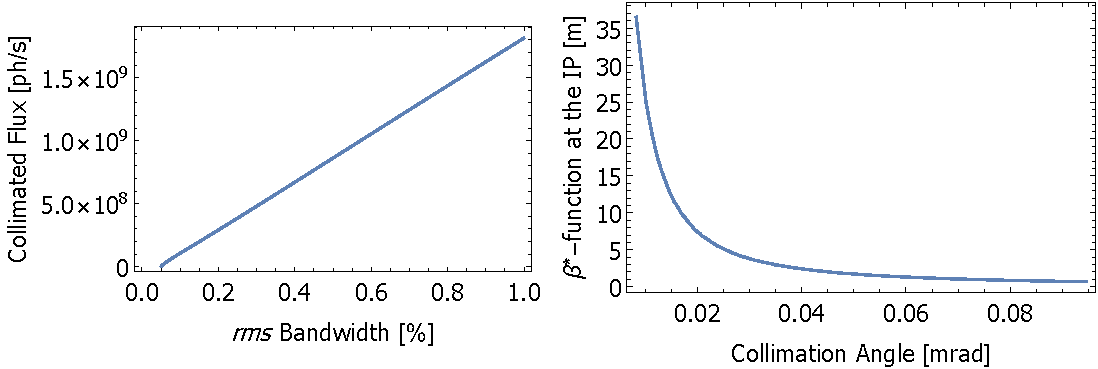
\includegraphics[width=\textwidth]{Figures/Optimisation_and_Characterisation_of_Inverse_Compton_Scattering_Sources/Case_A_RB_Tuning_Curves.pdf}
\caption{Case A (see Table~\ref{tab:char_opt_electron_bunch_parameters}) tuning curves in both solution space ($\mathcal{F}_{\mathrm{col}}$--$\left(\Delta E_{\gamma}/E_{\gamma}\right)_{\mathrm{rms}}$) and parameter space ($\beta^{*}$--$\theta_{\mathrm{col}}$), using the round beam optimisation method. Left: Solution space plot showing the Pareto-optimal front. Right: Parameter space plot showing the optimal variable front. Wide-band solutions favour large collimation angle and small $\beta$-function at the IP (collimation dominated), narrow-band solutions favour small collimation angle and and large $\beta$-function at the IP (emittance dominated).}
\label{fig:CaseA_RB_tuning_curve}
\end{figure}

Fig.~\ref{fig:CaseA_RB_tuning_curve} shows the Pareto-optimal front for the case A parameters within the \textit{rms} bandwidth range 0--1\%, which as previously defined is the regime of narrowband operation. A small bandwidth limitation of $\sim$0.05\% exists due to the electron bunch energy spread and laser spectral bandwidth of the source. The parameter space around this point is heavily restricted leading to a very small non-linear region. The non-linear region typically increases in size with larger values of the electron energy spread and laser pulse spectral bandwidth, hence it is minimal here. Beyond the non-linear region due to the low bandwidth limitation, the collimated flux appears to vary linearly with \textit{rms} bandwidth with collimated flux increasing, as expected, as the energy acceptance of the scattered photon beam increases.  

The $\beta^{*}$--$\theta_{\mathrm{col}}$ parameter space of the case A plot in Fig.~\ref{fig:CaseA_RB_tuning_curve} has a distinctive 'elbow shaped' front corresponding to the Pareto-optimal front. All solutions above this front are possible -- combinations of larger $\beta^{*}$-functions and collimation angles, and vice versa may give the same \textit{rms} bandwidth but will have lower collimated flux -- but the front shown is optimal in the round beam case. The more narrowband solutions typically lie at the higher $\beta$-function at the IP and smaller collimation angle part of the tuning curve whereas the wider-band soulutions exist at smaller $\beta$-functions at the IP and larger collimation angles. The small collimation angle and large $\beta$-function area of the tuning curve is the emittance dominated portion as the emittance term (Eq.~\ref{eq:emittance_term_round_beam}) is dominant, unlike in the wider-band, larger collimation angle and smaller $\beta^{*}$-function zone where collimation term dominates, named the collimation dominated portion. A stationary point exists in the tuning curve at which emittance domination switches to collimation domination, which whilst is not visible for case A is clear in case C (Fid.~\ref{fig:CaseC_RB_tuning_curve}). 


\begin{figure}[!h]
\centering
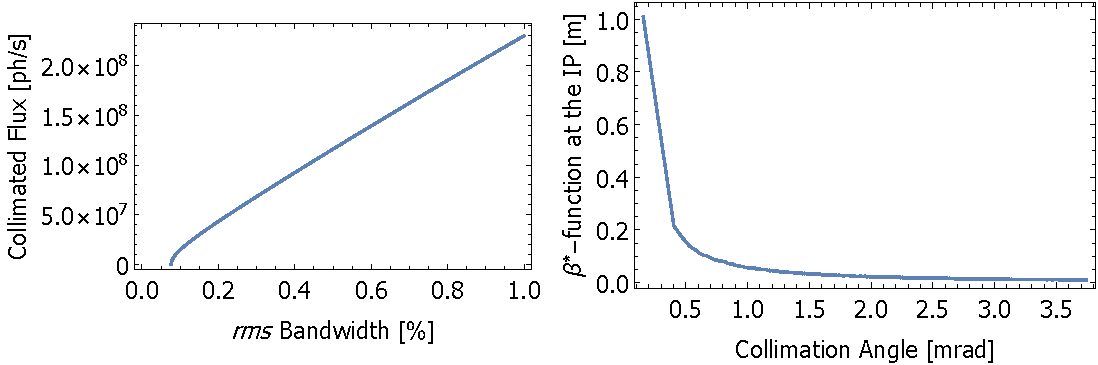
\includegraphics[width=\textwidth]{Figures/Optimisation_and_Characterisation_of_Inverse_Compton_Scattering_Sources/Case_C_RB_Tuning_Curves.pdf}
\caption{Case C (see Table~\ref{tab:char_opt_electron_bunch_parameters}) tuning curves in both solution space ($\mathcal{F}_{\mathrm{col}}$--$\left(\Delta E_{\gamma}/E_{\gamma}\right)_{\mathrm{rms}}$) and parameter space ($\beta^{*}$--$\theta_{\mathrm{col}}$), using the round beam optimisation method. Left: Solution space plot showing the Pareto-optimal front. Right: Parameter space plot showing the variable front corresponding to the Pareto-optimal front in solution space. Narrow-band solutions favour small collimation angle and and large $\beta$-function at the IP (emittance dominated), whereas wide-band solutions favour large collimation angle and small $\beta$-function at the IP (collimation dominated).}
\label{fig:CaseC_RB_tuning_curve}
\end{figure}

Fig.~\ref{fig:CaseC_RB_tuning_curve} shows the Pareto-optimal front in case C has an extended non-linear region around the X\% minimum achievable \textit{rms} bandwidth. Beyond the non-linear region, as in case A (Fig.~\ref{fig:case_A_GA_tuning_curves}), the collimated flux is related linearly to the \textit{rms} bandwidth. All collimated flux and \textit{rms} bandwidth combinations below the Pareto-optimal front in solution space are plausible.  

Case C RB parameter space, as shown in Fig.~\ref{fig:}, has the same overall characteristic 'elbow' shape of the parameter space front, however this is more severe -- the gradients in each of the regions is more variable. Distinction between the emittance dominated and collimation doiminated regions is more visible due to the smaller emittance. The case C stationary point in parameter space, where emittance dominance becomes collimation dominance, exists at around $\theta_{\mathrm{col}} = 0.35$~\si{\milli\radian} and $\beta^{*} = 0.20$~\si{\meter}. In the emittance dominated region there appears to be linear relationship between the variables, which is not present in Fig.~\ref{fig:CaseA_RB_tuning_curve}.

\section{2D Non-Round Beam Optimisation}
\label{sec:NRB_optimisation}

In a non-round beam (NRB) optimisation we relax the conditions that are imposed in the round beam case in Section~\ref{sec:RB_optimisation}, so that the transverse normalised emittances in each plane ($\epsilon_{nx}/\epsilon_{ny}$) and the $\beta$-functions at the IP in each direction ($\beta_{x}^{*}/\beta_{y}^{*}$) can differ, as well as the collimation angle. There are now three variables, unlike the two in the 1D RB case in Section~\ref{sec:RB_optimisation}. For a 2D non-round beam optimisation, the selected $\beta$-function variables can not be easily bound or calculated as a function of each other as in (Eq.~\ref{eq:beta_star_round_beam}) of the round beam methodology because of the form of the non-approximated emittance term (Eq.~\ref{eq:emittance_term}), which can not be re-arranged simply like the emittance term in the RB case (Eq.~\ref{eq:emittance_term_round_beam}). Therefore, the 2D non-round beam optimisation can't operate as a simple brute force optimisation method as in the RB optimisation.

The 2D NRB optimisation for the tuning curve case can be framed as a 3-dimensional, double objective non-linear minimisation problem of the form
\begin{equation}
\begin{aligned}
&\underset{\theta_{\mathrm{col}},~\beta_{x}^{*},~\beta_{y}^{*}}{\text{minimize}},  &-\mathcal{F}_{\mathrm{col}}\left(\theta_{\mathrm{col},~\beta_{x}^{*}},~\beta_{y}^{*}\right), \\
& &\left(\frac{\Delta E_{\gamma}}{E_{\gamma}}\right)_{\mathrm{rms}}\left(\theta_{\mathrm{col}},~\beta_{x}^{*},~\beta_{y}^{*}\right), \\
&\text{subject to} &0 < \theta_{\mathrm{col}} <  \theta_{\mathrm{col},\mathrm{max}}, \\
& &0 < \beta_{x}^{*} \leq \beta_{x,\mathrm{max}}^{*}, \\
& &0 < \beta_{y}^{*} \leq \beta_{y,\mathrm{max}}^{*}, 
\end{aligned}
\label{eq:2D_tuning_curve_optimisation_definition}
\end{equation}
\textcolor{blue}{**SORT OUT SPACING, number also in wrong place**}
where $\mathcal{F}_{\mathrm{col}}$ is the collimated flux (Eq.~\ref{eq:collimated_flux}) -- the neagative collimated flux is minimised therefore collimated flux is maximised -- and $\left(\Delta E_{\gamma}/E_{\gamma}\right)_{\mathrm{rms}}$ is the \textit{rms} bandwidth (Eq.~\ref{eq:RMS_bandwidth}) are the objective functions, $\theta_{\mathrm{col},\mathrm{max}}$ is the approximate upper bound on the collimation angle (Eq.~\ref{eq:collimation_angle_upper_bound}) and $\beta_{x/y,\mathrm{max}}^{*}$ are the upper bounds of the $\beta$-functions at the IP in each plane, which are set arbitrarily on a case by case basis. For single point optimisations, the problem is modified with the penalty function $\Omega$ (Eq.~\ref{eq:penalty_function}) instead of the \textit{rms} bandwidth, and the problem becomes
\begin{equation}
\begin{aligned}
&\underset{\theta_{\mathrm{col}},~\beta_{x}^{*},~\beta_{y}^{*}}{\text{minimize}},  &-\mathcal{F}_{\mathrm{col}}\left(\theta_{\mathrm{col},~\beta_{x}^{*}},~\beta_{y}^{*}\right), \\
& &\Omega\left(\theta_{\mathrm{col}},~\beta_{x}^{*},~\beta_{y}^{*}\right), \\
&\text{subject to} &0 < \theta_{\mathrm{col}} <  \theta_{\mathrm{col},\mathrm{max}}, \\
& &0 < \beta_{x}^{*} \leq \beta_{x,\mathrm{max}}^{*}, \\
& &0 < \beta_{y}^{*} \leq \beta_{y,\mathrm{max}}^{*}, 
\end{aligned}
\label{eq:2D_single_point_optimisation_definition}
\end{equation}
\textcolor{blue}{**SORT OUT SPACING, number also in wrong place**}
Due to the complexity of the 2D NRB optimisation problems, a more sophisticated approach  to solving the optimisation problems than in the RB case (Section~\ref{sec:RB_optimisation}) is required. Two optimisation methodologies are employed to solve this: a genetic algorithm approach, developed in collaboration with Prof B. Terzic, and a downhill simplex approach, which are detailed in the following section and are compared in Section~\ref{sec:evaluation_of_optimisation_methods}.

\subsection{Genetic Algorithm Approach}

% Point heavily to SPEA2 paper etc.
% Just want to give an overview of how these things work
% Fitness, Mating, Strength etc. -> what happens?
% define feasible, non-dominated, individual, generation etc.
In a genetic algorithm, a set of individuals -- a single point in multi-dimensional parameter space -- known as a population are randomly generated in the bounded parameter space; all of these points are feasible solutions to the optimisation problem. The objective functions are then calculated for each individual based on these variables, a fitness function which is dependent on the objective functions is then evaluated which measures how well an individual meets the optimization goals \cite{hofler2013innovative}. The design of fitness functions vary greatly between different genetic algorithms. The individuals are then evaluated against eachother via a competition -- typically a head to head fitness comparison between pairs of individuals -- where the fitter (higher fitness) individuals that beat the other individuals are selected to form a subset named the mating pool. The mating pool is the set of individuals which dominate (beat) other individuals in the population and aren't dominated by any other individual -- they are non-dominated. The mating pool individuals are the subset of the population which will form the next generation, which is the new population of the next iteration. In most GA's some non-dominated points of the previous generation are also inducted into the next generation. Individuals in the mating pool are paired together \textcolor{blue}{**HOW**} and through recombination -- exchanging of variable values -- and mutation -- adjustment (scaling) of single parameter space variables \cite{hofler2013innovative} -- designed to mimic biological reproduction a set of new individuals for the next generation, named offspring, are produced.

Therefore, a genetic algorithm operates with a general basic procedure to solve a multi-dimensional multi-objective optimisation problem:
\begin{enumerate}
    \item{A population of individuals are randomly generated to sample the parameter space.}
    \item{Objective and fitness functions are evaluated for each individual in the new generation}
    \item{All non-dominated individuals of the previous generation are introduced (step doesn't apply in generation 1). }
    \item{If a termination condition is met, for example the no. generations exceeds a pre-set value, the simulation stops and the non-dominated individuals make up the Pareto front. }
    \item{A form of competition is used to select candidates to form the mating pool, which decides the composition of individuals in the next generation.}
    \item{Individuals in the mating pool are paired together \textcolor{blue}{**HOW? RANDOMLY DOESN'T SEEM RIGHT?} and these produce the individuals of the next generation via recombination and mutation}
    \item{A new generation begins. The simulation is iterated starting from step 2. This repeats until the termination condition in step 4 is satisfied.}
\end{enumerate}
Once the termination condition has been satisfied, the Pareto-optimal front has been deciphered and the parameters of all of the non-dominated individuals that constructed the Pareto-optimal front are returned. 

The genetic algorithm method is a global optimisation technique which provides a set of solutions for each optimisation run, allowing the full solution space to be mapped more effectively. Optimisation via a genetic algorithm delivers a global maximum for the collimated flux at each of the \textit{rms} bandwidths or values of the penalty function within the limits of the variables. This method should avoid the pitfalls of local optimisation techniques where a local minima may be returned however, this comes at the cost of longer optimisation times. If the parameter space is simple the GA method may also be overly sophisticated for the problem and less complicated optimisation may return a similar accuracy and precision result. Termination conditions and many other parameters, such as the number of individuals, have been set abitrarily within this method or to the values used by Hofler et al \cite{hofler2013innovative}. For example, the simulation terminates arbitrarily after 200 generations and 50 individuals are used as a balance between optimisation time and good coverage of the parameter space. Full benchmarking of each simulation parameter for a GA is extensive and, for the method chosen here, is beyond the scope of this work. 

The genetic algorithm (GA) optimisation uses the minimisation routine of \textsc{SPEA2} \cite{zitzler2001spea2} within the \textsc{PISA} platform \cite{bleuler2003pisa} framework, following the methodology outlined by A. Hofler et al \cite{hofler2013innovative}. The \textsc{SPEA2} algorithm is a multiobjective evolutionary algorithm which incorporates a fine grained fitness assignment strategy \cite{zitzler2001spea2} with density evaluation, using an archive of non-dominated points from previous generations to supplement determination of the mating pool of the current generation. In the \textsc{SPEA2} algorithm, the fitness function is defined by
\begin{itemize}
    \item{Assigning each individual a strength value representative of the number of solutions it dominates.}
    \item{Defining raw fitness based upon the strength value of the current population and archived population.}
    \item{Calculating a density function for each individual, using the $k$th nearest neighbour method \cite{silverman1986density}, which is introduced as raw fitness can fail when most individuals don't dominate eachother for example, when there are many objectives.}
    \item{The fitness is then defined as the raw fitness plus the density.}
\end{itemize}
A full explanation of the fitness determination is omitted for brevity, and is better described by Zitzler et al \cite{zitzler2001spea2} where a full explanation of the \textsc{SPEA2} algorithm is given. The \textsc{SPEA2} fitness function enables the non-dominated Pareto-optimal set to be determined more efficiently and reliably.

The developed GA utilises a set of \textsc{Python} calculation scripts designed to calculate the values of the objective functions are implemented on the \textsc{PISA} platform \cite{bleuler2003pisa},  templates have been produced to allow for simulation of different ICS sources and the platform has been configured for three variables and two objective functions. The upper and lower limits of the variables are imposed in a configuration file and are set as mentioned in (Eqs.~\ref{eq:2D_tuning_curve_optimisation_definition}, \ref{eq:2D_single_point_optimisation_definition}) with the upper bound of the $\beta$-functions at the IP imposed arbitrarily at a large value in the 10's~\si{\meter} and the collimation angle limited by (Eq.~\ref{eq:collimation_angle_upper_bound}) for a user selected bandwidth or bandwidth upper bound. The GA optimises the multi-dimensional multi-objective minimisation problems outlined in (Eqs.~\ref{eq:2D_tuning_curve_optimisation_definition},~\ref{eq:2D_single_point_optimisation_definition}) where, as both optimisation problems have conflicting objectives, multiple equally valid solutions exist in the solution space which define a Pareto-optimal front. Each solution on the Pareto-optimal front is a feasible solution, non-dominated with respect to other individuals that contribute to the Pareto front and dominates another feasible individual in the solution space \cite{hofler2013innovative}. The Pareto-front non-dominated individual data (variable and objective function valies) is wrote to file as well as all the data of the individuals trialed within the course of the optimisation.  

In the case of the tuning curve optimisation, the Pareto-optimal front that is defined in solution space is the tuning curve; the Pareto-optimal front shows the maximal collimated flux for each \textit{rms} bandwidth constrained by the variable limits. Whereas, in the single point optimisations a Pareto-optimal front of the collimated flux as a function of the penalty function is returned. Therefore, the single optimal solution is decided in a post-processing selection procedure by isolating all values that fit the penalty function criteria of $\Omega < 10^{-5}$, used as this is well below experimental tolerances \textcolor{blue}{**JUSTIFY**}, and selecting the solution with the maximal collimated flux. The selection procedure is advantageous over choosing the point with the minimum penalty function as this accounts for anomalous collimated flux deficient points near $\Omega = 0$, which can occur due to a lack of individuals achieving a small penalty function.          

By inspection of the variables in parameter space corresponding to the non-dominated Pareto-optimal individuals in solution space, relationships can be deduced. Characteristics of the Pareto-optimal variables parameter space, such as stratification of the points can show that some variables have more influence over the objective functions than others. For example, a lesser spread in the Pareto-optimal variable vales of $\theta_{\mathrm{col}}$ compared to $\beta_{x}^{*}$ would suggest that $\theta_{\mathrm{col}}$ is a more important variable to the optimisation. In single point optimisations, the pareto-optimal variables of the selected point are the optimal configuration for the ICS source.  

The genetic algorithm approach has been applied to each of the electron bunch parameter cases in Table~\ref{tab:char_opt_electron_bunch_parameters} using the laser parameters in Table~\ref{tab:char_opt_laser_pulse_parameters} using a population of 50 individuals and spanning the optimisation over 200 generations. Plots of the tuning curves produced via the genetic algorithm method are shown in Figs.~\ref{fig:case_A_GA_tuning_curves}, \ref{fig:case_B_GA_tuning_curves} and \ref{fig:case_C_GA_tuning_curves}, demonstrating the typical output of the genetic algorithm where the non-dominated Pareto front points are highlighted and the other trial points are shown. Onward from this section in the thesis only the Pareto front points and their corresponding variables will be included in plots to aid comparison of optimisation methods.

\begin{figure}[!h]
\centering
\includegraphics[width=\textwidth]{Figures/Optimisation_and_Characterisation_of_Inverse_Compton_Scattering_Sources/CaseA_GA_Tuning_Curve.pdf}
\caption{Case A genetic algorithm tuning curves (solution and parameter space) produced using 200 generations and 50 individuals showing the non-dominated Pareto front points (red) and the dominated trial points (blue). Top Left: collimated flux as a function of \textit{rms} bandwidth solution space. Top Right: parameter space plot of the $\beta$-function in the $x$ plane as a function of the $\beta$-function in the $y$ plane at the IP. Bottom Left: parameter space plot of the $\beta_{x}$-function at the IP as a function of the collimation angle. Bottom Right: parameter space plot of the $\beta_{y}$-function at the IP as a function of the collimation angle.}
\label{fig:case_A_GA_tuning_curves}
\end{figure}

In Fig.~\ref{fig:case_A_GA_tuning_curves}, we see a clearly defined Pareto-optimal front in the collimated flux--\textit{rms} bandwidth solution space. The individuals that construct the solution space Pareto-optimal front are clearly non-dominated with a series of dominated points shown below this front. The resulting Pareto-optimal front is clearly the maximal collimated flux as a function if \textit{rms} bandwidth, and therefore a tuning curve for the case A ICS source. The $\beta_{x}^{*}$--$\beta_{y}^{*}$ parameter space plot shows that the variables corresponding to the non-dominated solutions do not follow the round beam solution ($\beta_{x}^{*}=\beta_{y}^{*}=\beta^{*}$), therefore non-round beam simulation is beneficial in all cases even when $\epsilon_{nx}=\epsilon_{ny}=\epsilon_{n}$ -- as is necessary for the RB optimisation -- as this is observed by case A. Typically, the Pareto-optimal variables favour $\beta_{x}^{*}>\beta_{y}^{*}$; the only possible explanation is that this is because the crossing angle is impose in the $x$--$z$ plane because this is the only difference between the two planes. Many dominated individuals exist around the parameter space of the Pareto-optimal individuals in the $\beta_{x}^{*}$--$\beta_{y}^{*}$ parameter space, demonstrating that the parameter space is well explored.

The parameter spaces  of the $\beta$-functions against the collimation angle show very different relationships in the Pareto-optimal variables due to the crossing angle in the $x$--$z$ plane. The $\beta_{x}$--$\theta_{\mathrm{col}}$ parameter space shows a large stratification in the Pareto-optimal variable positions which shows that the objective functions have a weak dependence on this variable, this plot varies largely from the $\beta^{*}$--$\theta_{\mathrm{col}}$ parameter space curve in Fig.~\ref{fig:CaseA_RB_tuning_curve}. In comparison, the $\beta_{y}^{*}$--$\theta_{\mathrm{col}}$ parameter space plot shows far less stratification of the Pareto-optimal front variables and this also mirrors the elbow shape of the optimal variables in the parameter space of the RB optimisation in Fig.~\ref{fig:CaseA_RB_tuning_curve}. In both of the $\beta$-function at the IP against collimation angle parameter space plots for case A there appears to be a lack of statistics -- dominated points -- around 0.02~\si{\milli\radian}, the cause of which is unknown though this may be a random occurrence in the optimisation.    

\begin{figure}[!h]
\centering
\includegraphics[width=\textwidth]{Figures/Optimisation_and_Characterisation_of_Inverse_Compton_Scattering_Sources/CaseB_GA_Tuning_Curve.pdf}
\caption{Case B genetic algorithm tuning curves (solution and parameter space) produced using 200 generations and 50 individuals showing the non-dominated Pareto front points (red) and the dominated trial points (blue). Top Left: collimated flux as a function of \textit{rms} bandwidth solution space. Top Right: parameter space plot of the $\beta$-function in the $x$ plane as a function of the $\beta$-function in the $y$ plane at the IP. Bottom Left: parameter space plot of the $\beta_{x}$-function at the IP as a function of the collimation angle. Bottom Right: parameter space plot of the $\beta_{y}$-function at the IP as a function of the collimation angle.}
\label{fig:case_B_GA_tuning_curves}
\end{figure}

Within the GA simulation of the case B tuning curve in Fig.~\ref{fig:case_B_GA_tuning_curves}, the Pareto-optimal front in the collimated flux--\textit{rms} bandwidth is well defined, showing only non-dominated individuals, with an increase in flux of a factor $\sim2$ on the case A parameters in Fig.~\ref{fig:case_A_GA_tuning_curves} for a 1\% \textit{rms} bandwidth, though this simulation is extended to 3\% as the case B parameters are more conducive to wider bandwidth operation. In the $\beta_{x}^{*}$--$\beta_{y}^{*}$ parameter pace, the Pareto-optimal variables clearly favour a large $\beta_{x}^{*}$ over $\beta_{y}^{*}$, the stratification in the Pareto-optimal variables is much less that that for case A. The $\beta$-function at the IP against collimation angle parameter space plots in Fig.~\ref{fig:case_B_GA_tuning_curves} differ more so between each plane than those in case A (Fig.~\ref{fig:case_A_GA_tuning_curves}) due to the non-symmetry of the emittance in each plane. In the $\beta_{x}^{*}$--$\theta_{\mathrm{col}}$ parameter space the Pareto-optimal variables are stratified as in Fig.~\ref{fig:case_A_GA_tuning_curves}, however in case B many variables exist at the upper bounds of both the collimation angle and $\beta_{x}^{*}$-function as the $\beta^{*}$-function at the IP has been arbitrarily limited. In the $\beta_{y}^{*}$--$\theta_{\mathrm{col}}$ parameter space the typical 'elbow' shape seen in the round beam optimisations is more evident, and the Pareto-optimal variables are less stratified however there seems to be an unusual lack of individuals around $5\mathrm{~\si{m}} < \beta_{y}^{*} < 10\mathrm{~\si{m}}$ which is unexplained.

\begin{figure}[!h]
\centering
\includegraphics[width=\textwidth]{Figures/Optimisation_and_Characterisation_of_Inverse_Compton_Scattering_Sources/CaseC_GA_Tuning_Curve.pdf}
\caption{Case C genetic algorithm tuning curves (solution and parameter space) produced using 200 generations and 50 individuals showing the non-dominated Pareto front points (red) and the dominated trial points (blue). Top Left: collimated flux as a function of \textit{rms} bandwidth solution space. Top Right: parameter space plot of the $\beta$-function in the $x$ plane as a function of the $\beta$-function in the $y$ plane at the IP. Bottom Left: parameter space plot of the $\beta_{x}$-function at the IP as a function of the collimation angle. Bottom Right: parameter space plot of the $\beta_{y}$-function at the IP as a function of the collimation angle.}
\label{fig:case_C_GA_tuning_curves}
\end{figure}

The GA tuning curves for case C in Fig.~\ref{fig:case_C_GA_tuning_curves} shows a well defined Pareto-optimal front in collimated flux--\textit{rms} bandwidth space which shows the case C ICS source is capable of narrowband operation with a minimum \textit{rms} bandwidth of $\sim0.1$\%. Pareto-optimal variables in the $\beta$-function in each plane parameter space are clustered either at small values or around $\beta_{x}^{*} = 14$~\si{\meter}, $\beta_{y}^{*} = 8$~\si{\meter}, which is unexpected but still shows that generally $\beta_{x}^{*}>\beta_{y}^{*}$ is preferred. Pareto-optimal variables in the $2\mathrm{~\si{\meter}} < \beta_{x}^{*} < 11\mathrm{~\si{\meter}}$ range of the $\beta_{x}^{*}$--$\theta_{\mathrm{col}}$ parameter space plot are sparse; this area of the parameter space has been poorly explored. Variation in the number of individuals simulated may improve statistics in this region. The $\beta_{y}^{*}$--$\theta_{\mathrm{col}}$ parameter space plot shows that individuals on the tuning curve in solution space favour small $\beta_{y}^{*}$-functions at large collimation angle until a sharp transition at $\sim0.2$~\si{\milli\radian}, however the Pareto-optimal variables do adhere to the 'elbow' shape of the round beam plots in Fig.~\ref{fig:CaseC_RB_tuning_curve}. The $\beta_{x}^{*}$--$\beta_{y}^{*}$ parameter space plot shows that typically larger $\beta$-functions are favoured in the $x$-plane than the $y$-plane however, there is clustering of Pareto-optimal variables around $\beta_{x}^{*} = 14$~\si{\meter} and $\beta_{y}^{*} = 8$~\si{\meter} which is explained by the very narrow bandwidth emittance dominated solutions.

\subsection{Simplex Approach}

\textcolor{blue}{**HOW DOES SIMPLEX OPTIMISATION WORK**}

The downhill simplex method is a direct search optimisation method used to minimise an objective function $f\left(x\right)$, where for a function of $n$ variables a set of $n+1$ points ($x_{1}$--$x_{n+1}$) are used to form the vertices of a polytope in $n$-dimensional space \cite{wolfram2021nmaximize}. For example, in the 2D NRB optimisation there are 3 variables so the polytope is a 4-vertex polyhedron in parameter space. Selection of
the vertex points can be prescribed, but random selection allows the potential to fully investigate the parameter space \cite{koshel2002enhancement}. Here the simplex method will be explained using the Wolfram \textsc{Mathematica} formalism \cite{wolfram2021nmaximize}. The objective function is calculated for each of these vertex's and they are sorted into the form
\begin{equation}
f\left(x_{1}\right) \leq f\left(x_{2}\right) \leq \ldots \leq f\left(x_{n+1}\right),
\label{eq:simplex_polytope_objective_functions}
\end{equation}
where their order is from minimum objective function ($x_{1}$, best point) to maximum objective function ($x_{n+1}$, worst point). The worst point is then replaces in the set by a trial point $x_{t}$, given by
\begin{equation}
x_{t} = c+s_{r}\left(c-x_{n+1}\right),
\label{eq:simplex_trial_point}    
\end{equation}
which is a reflection of the worst point $x_{n+1}$, with $s_{r} > 0$ the refection parameter and the midpoint $c$ of the n-dimensional polytope is given by
\begin{equation}
c = \frac{1}{n}\sum_{i=1}^{n}x_{i}.
\label{eq:polytope_centroid_simplex}
\end{equation}

If $\x_{t}$ minimises the objective better than the best point ($f\left(x_{t}\right) \leq f\left(x_{1}\right)$), then reflection is a successful method in minimising the objective function. The effect of the reflection may be accentuated by an expansion of the polytope in that direction via the trial point $x_{e}$ given by
\begin{equation}
x_{e} = c+s_{e}\left(x_{t}-c\right),
\label{eq:simplex_expansion}    
\end{equation}
where $s_{e} > 1$ is the expansion parameter. If $f\left(x_{e}\right) < f\left(x_{t}\right)$, $x_{e}$ is a better solution and then replaces the worst point in the set $x_{n+1}$, otherwise $x_{t}$ replaces $x_{n+1}$. 

A more optimal vertex may then be found via a contraction of the polytope if the new trial point $x_{t}$ is worse than the the second worst point $f\left(x_{t}\right) \geq f\left(x_{n}\right)$, the new trial vertex is given by
\begin{equation}
x_{c} = 
\begin{cases}
c+s_{c}\left(x_{n+1}-c\right), & \text{if}  ~f\left(x_{t}\right) \geq f\left(x_{n+1}\right), \\
c+s_{c}\left(x_{t}-c\right), & \text{if}  ~f\left(x_{t}\right) < f\left(x_{n+1}\right),
\end{cases}
\label{eq:simplex_contraction}
\end{equation}
where $0 < s_{c} < 1$ is the contraction parameter. A further contraction, named a shrink is carried out if $f\left(x_{c}\right) < f\left(x_{n+1}\right) \land f\left(x_{t}\right)$ because the previous contraction was successful, with $x_{t}$ replacing $x_{n+1}$. A shrink would be of identical form to (Eq.~\ref{eq:simplex_contraction}) with the contraction parameter $s_{c}$ replaced by a shrink parameter $0 < s_{s} < 1$ 

The method is then iterated until the termination condition, typically a number of iterations, is exceeded or until convergence below a set tolerance in the penalty function (Eq.~\ref{eq:penalty_function}) is achieved. 

\textcolor{blue}{**CONSTRAINTS IN SIMPLEX?**}

\textcolor{blue}{**WHY IS simplex USEFUL + NOT**}
The simplex methodology is typically a fast optimisation process because a minimum of $n+1$  objective function calculations, with $n$ variables, are required per iteration in comparison to genetic algorithm methods where objective functions are calculated for each individual. Since a single trial point is compared against $n+1$ points in each iteration, the comparative aspect of a downhill simplex method is also more efficient. The combination of these factors mean the downhill simplex method can be a fast optimisation, on the scale of minutes for the single point optimisation examples. A full benchmarking of the simplex method is also more readily achievable due to the small number of simulation settings that can be adjusted -- these consist of the 4 constants governing refection and expansion etc., the tolerance of the simulation and the no. iterations.   

The downhill simplex optimisation method is a local minimisation routine as effectively, derivatives are used to find minima \cite{jones2016design} therefore, unlike in the GA method, only a single solution space point is returned for each optimisation. This means the full solution space is not mapped in this optimisation. The simplex optimisation may also fail to find the optimal solution and become trapped in a local minima as this is a heuristic method, however in practice downhill simplex tends to work reasonably well for problems that do not have many local minima \cite{wolfram2021nmaximize}. The parameter space of the 2D NRB optimisation problem (Eq.~\ref{eq:2D_tuning_curve_optimisation_definition}) is assumed to be simple enough to produce a global minima result, however this assumption will be evaluated in Section~\ref{sec:evaluation_of_optimisation_methods} by comparison with the GA 2D NRB method. Another limitation of this method is that the optimisation arbitrarily terminates after a set number of iterations, which may mean that a true optimal solution is not found if finding it exceeds the iteration limit.

\textcolor{blue}{**HOW DOES THE CODE WORK**}

Within the simplex optimisation, the collimated flux (Eq.~\ref{eq:collimated_flux}) objective function is maximised and the bandwidth penalty function (Eq.~\ref{eq:penalty_function}) is minimised. In order to produce tuning curves using the simplex method, the optimisation is applied to an array of bandwidth values, as it is for the RB optimisation in Section~\ref{sec:RB_optimisation}.

The optimisation operates using the \textsc{NMaximise} maximisation routine in \textsc{Mathematica} \cite{wolfram2021nmaximize} using the simplex method built into this function. The collimated flux is set as the objective to be maximised whilst the condition to be satisfied is $\Omega = 0$ i.e the penalty function (Eq.~\ref{eq:penalty_function}) must equal zero within a tolerance of $10^{-5}$, analagous to the single point GA optimisation in Section~\ref{sec:}. The interaction point $\beta$-functions and collimation angle are initialised as variables, therefore the optimisation problem is stated as in (Eq.~\ref{eq:2D_single_point_optimisation_definition}) with the collimation upper bound given by (Eq.~\ref{eq:collimation_angle_upper_bound}).

\textcolor{blue}{**HOW DOES NMaximise WORK?**}
The NMaximise function aims to produce a global maximum, via minimising the inverse of the objective function i.e. minimising $-\mathcal{F}_{\mathrm{col}}$ subject to the $\Omega = 0$ penalty function (Eq.~\ref{eq:penalty_function}) constraint with a small tolerance ($\Omega < 10^{-5}$) subject to the other bounds on the variables; the arbitrary $\beta$-function at the IP in each plane upper bounds and the collimation angle upper bound (Eq.~\ref{eq:collimation_angle_upper_bound}). The downhill simplex method, detailed earlier in this section, is applied to minimise the negative collimated flux with 200 maximum iterations. The ReflectRatio, ExpandRatio, ContractRatio and ShrinkRatio parameters \textcolor{blue}{**MENTION THAT THESE CORRESPOND TO THE CONSTANTS**} \cite{wolfram2021nmaximize} of the simplex method are set to their default values as this was found to be sufficient to optimise all of the cases in Table~\ref{tab:char_opt_electron_bunch_parameters}.

\textcolor{blue}{**RESULTS**}
\textcolor{blue}{\textbf{**SHOW PLOTS OF THE 3 CASES TUNING CURVES (Fcol-rmsBW)**} \\ **TALK ABOUT THESE PLOTS** \\ **TRY TO REMEDY THE SHIT CASE C**}
The results of the simplex NRB tuning curve optimisations are shown in Fig.~\ref{fig:case_A_simplex_tuning_curves}, \ref{fig:case_B_simplex_tuning_curves} and \textcolor{blue}{**CASE C**}, produced using 200 iterations and the \textsc{Mathematica} \cite{wolfram2021nmaximize} default values of the simplex scaling parameters ($s_{r}$, $s_{e}$, $s_{c}$, $s_{s}$) in the optimisation. The collimation angle is upper bounded by (Eq.~\ref{eq:collimation_angle_upper_bound}), with a lower bound of $\theta_{\mathrm{col}} > 0$. The $\beta$-functions at the IP are upper bounded by  $\beta_{x/y}^{*} < 20~\mathrm{\si{\meter}}$ with the exception of case B where the upper bound of the $\beta_{x}$, which is given by $\beta_{x}^{*} < 100$~\si{\meter}. The lower bounds of the $\beta$-functions at the IP are set \textit{a posteriori} to $\beta_{x/y}^{*} > 1$~\si{\milli\meter}, as this appears to be a reasonable limitation of simple final-focusing systems like those that would be imposed within most ICS sources. 

\begin{figure}[!h]
\centering
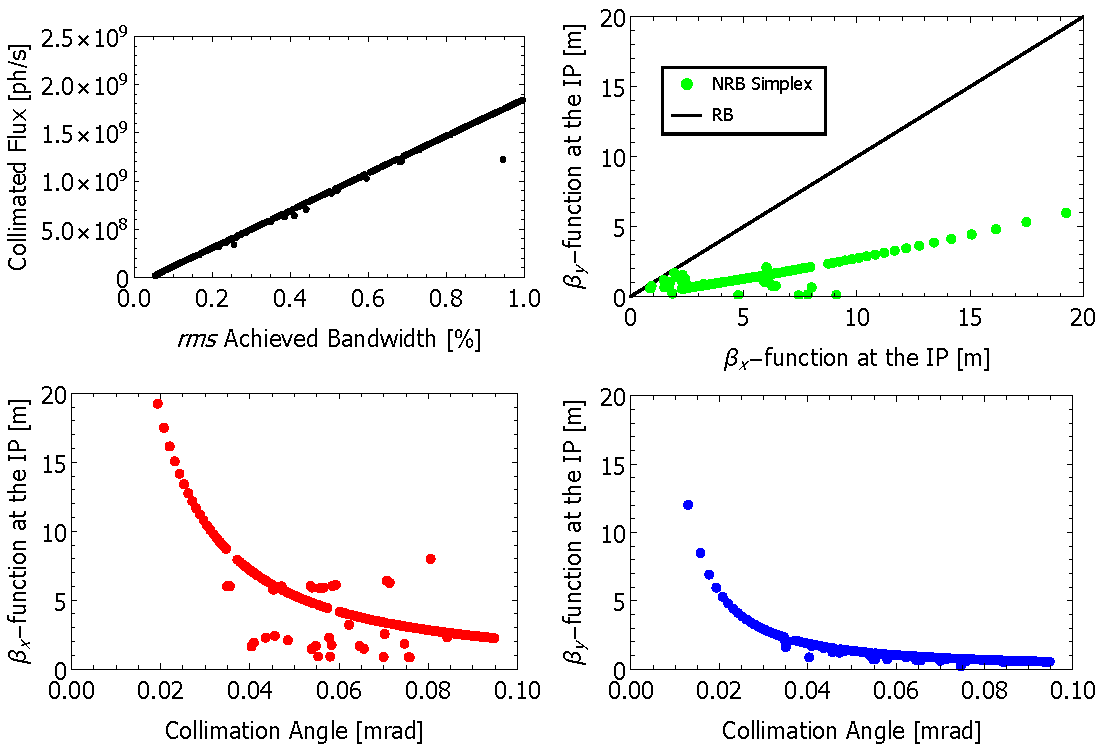
\includegraphics[width=\textwidth]{Figures/Optimisation_and_Characterisation_of_Inverse_Compton_Scattering_Sources/Case_A_simplex_Tuning_Curves.pdf}
\caption{Case A simplex optimisation tuning curves in both solution and parameter space. Top Left: Pareto-optimal front of the collimated flux as a function of \textit{rms} bandwidth. Top Right: Simplex parameter space ($\beta_{x}^{*}$--$\beta_{y}^{*}$) variable front (green) corresponding to the Pareto-optimal front in solution space compared to the monotonically varying round beam variable front (black). Bottom Left: Parameter space ($\beta_{x}^{*}$--$\theta_{\mathrm{col}}$) corresponding to the Pareto-optimal front in solution space. Bottom Right: Parameter space ($\beta_{y}^{*}$--$\theta_{\mathrm{col}}$) corresponding to the Pareto-optimal front in solution space.}
\label{fig:case_A_simplex_tuning_curves}
\end{figure}

The Pareto-optimal front in solution space ($\mathcal{F}_{\mathrm{col}}$--$\left(\Delta E_{\gamma}/E_{\gamma}\right)_{\mathrm{rms}}$) in Fig.~\ref{fig:case_A_simplex_tuning_curves} using the simplex NRB method is well defined in the 0--1\% \textit{rms} bandwidth range. The minimum achieved bandwidth is around $\sim0.05$\%, as in the RB case in Fig.~\ref{fig:CaseA_RB_tuning_curve}. Convergence to local minima solutions appears to occur for several points in solution space; the complexity of solution space is minimal, and the downhill simplex method is generally satisfactory for case A.    

The $\beta_{x}^{*}$--$\beta_{y}^{*}$ parameter space plot corresponding to the Pareto-optimal front shows that the optimal solution is a non-round transverse electron bunch profile at the interaction point. The $\beta_{x}^{*}$-function is typically larger than the $\beta_{y}^{*}$ function in Fig.~\ref{fig:case_A_simplex_tuning_curves} which means a larger horizontal transverse profile is favoured. As the transverse emittance in each plane is identical, the favoured larger horizontal transverse profile can only be explained because of the non-zero crossing angle between the laser pulse and electron bunch in the $x$--$z$ plane. Both the $\beta$-function at the IP against collimation angle parameter space plots display the typical elbow shape observed in the RB case, as shown in Fig.~\ref{fig:CaseA_RB_tuning_curve}. However the $\beta_{x}^{*}$--$\theta_{\mathrm{col}}$ plot contains numerous off-trend Pareto-front corresponding points which lay in the range $0.03~\textrm{\si{\milli\radian}} < \theta_{\mathrm{col}} < 0.09~\mathrm{\si{\milli\radian}}$, which suggests the $\beta_{x}^{*}$ variable has a weak dependence on collimated flux and the weak dependence of this variable may be responsible for the non-optimal points in solution space.  

\begin{figure}[!h]
\centering
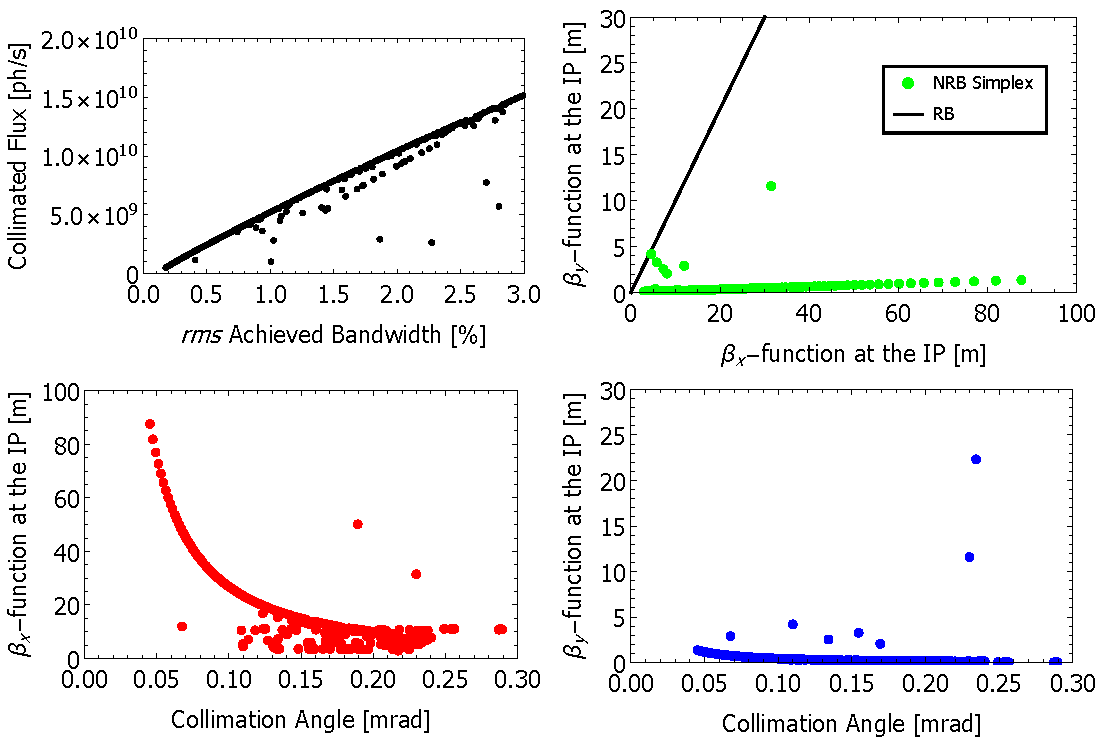
\includegraphics[width=\textwidth]{Figures/Optimisation_and_Characterisation_of_Inverse_Compton_Scattering_Sources/Case_B_simplex_Tuning_Curves.pdf}
\caption{Case B simplex optimisation tuning curves in both solution and parameter space. Top Left: Pareto-optimal front of the collimated flux as a function of \textit{rms} bandwidth. Top Right: Simplex parameter space ($\beta_{x}^{*}$--$\beta_{y}^{*}$) variable front (green) corresponding to the Pareto-optimal front in solution space compared to the monotonically varying round beam variable front (black). Bottom Left: Parameter space ($\beta_{x}^{*}$--$\theta_{\mathrm{col}}$) corresponding to the Pareto-optimal front in solution space. Bottom Right: Parameter space ($\beta_{y}^{*}$--$\theta_{\mathrm{col}}$) corresponding to the Pareto-optimal front in solution space.}
\label{fig:case_B_simplex_tuning_curves}
\end{figure}

Fig.~\ref{fig:case_B_simplex_tuning_curves} shows the Pareto-optimal front in solution space (collimated flux against \textit{rms} bandwidth) of the case B ICS source parameters in a 0--3\% \textit{rms} bandwidth range. The Pareto optimal front is well defined, however there are more anomalous points which don't adhere to the trend of the Pareto-front than in case A (see Fig.~\ref{fig:case_A_simplex_tuning_curves}). Therefore, in case B the downhill smiplex optimisation method is worse at finding a global maximum. The general linear relationship of increasing collimated flux with wider bandwidth is maintained, as in the genetic algorithm case in Fig.~\ref{fig:case_B_GA_tuning_curves}, as well as the presence of the minimum bandwidth limitation caused by the energy spread of the electron bunch and the laser pulse spectral bandwidth.

The parameter space tuning curve of the $\beta$-functions at the interaction point corresponding to the Pareto-optimal front show that the optimal configuration for radiation production in the 0--3\% \textit{rms} bandwidth is a non-round electron bunch transverse profile. The $\beta$-function in the $x$-plane is much larger than the $\beta$-function in the $y$ plane, for example at extreme emittance dominated narrow band case ($\beta_{x}^{*}\sim87$~\si{\meter}, $\beta_{y}^{*} \sim1$~\si{\meter}) the transverse electron bunch profile radius is $\sigma_{x,e} =1.09$~\si{\milli\meter} in the $x$ plane, and $\sigma_{y,e} =13.03$~\si{\micro\meter} in the $y$ plane-- a factor of $\sim100$ smaller.

The parameter space optimal front in Fig.~\ref{fig:case_B_simplex_tuning_curves} shows the typical elbow shape for the $\beta_{x}^{*}$--$\theta_{\mathrm{col}}$ tuning curve, however many solutions exist for $\theta_{\mathrm{col}} > 0.1$~\si{\milli\radian} which differ from the trend. The solutions that vary from the trend could be a signal of insensitivity of the optimisation to $\beta_{x}^{*}$ or are the result of local minima within the optimisations. The elbow shape is not visible due to the small optimal $\beta_{y}^{*}$ values in the $\beta_{y}^{*}$--$\theta_{\mathrm{col}}$ parameter space. High $\beta_{y}^{*}$ solutions are not beneficial for producing narrowband radiation in the emittance dominated regime because the $x$-plane interaction dynamics dominate due to the larger emitttance. Solutions are visible in $\beta_{y}^{*}$--$\theta_{\mathrm{col}}$ which are anomalies in the overall trend. 

\textcolor{blue}{**SORT OUT CASE C**}

\section{Evaluation of Optimisation Methods} 
\label{sec:evaluation_of_optimisation_methods}

Optimisations have been performed for each of the cases in Table~\ref{tab:char_opt_electron_bunch_parameters} using the laser parameters in Table~\ref{tab:char_opt_laser_pulse_parameters} using the RB (Section~\ref{sec:RB_optimisation}), GA NRB and simplex NRB (Section~\ref{sec:NRB_optimisation} methods. Since case B electron bunch parameters don't fulfill the round beam optimisation criteria ($\epsilon_{nx} = \epsilon_{ny} = \epsilon_{n}$) it has been excluded from these methods. Within this section the optimisation methods will be compared through both single point and tuning curve optimisations, to study the effect of optimisation hollistically towards narrowband radiation production, quantify the advantage of higher dimensional optimisation (from round to non-round transverse profiles) and examine the feasibility of each optimisation method. The reality of applying these optimisation techniques in practice requires further studies; for example accelerator jitter may impede the achievement of the optimised electron bunch transverse profile at the interaction point and the effect of this error on source performance needs to be quantified.   


\textcolor{blue}{**EVALUATE WHETHER simplex METHOD WORKS AS A GLOBAL OPTIMISER IN THIS CASE** \\ **MENTION THAT FURTHER WORK NEEDS TO BE CONDUCTED INTO HOW ACHIEVABLE THIS IS IN AN ICS SOURCE - JITTER + ERROR STUDIES** \\}

\subsection{Single Point Bandwidth Optimisations}

Single point bandwidth optimisations have been used to compare optimisation methods at small \textit{rms} bandwidths, 0.5\% \texit{rms} bandwidth for case A and C and 2\% \texit{rms} bandwidth for case B, to quantify the advantage of using each method and for comparison against the standard transverse profile matching approach in Section~\ref{sec:transverse_profile_matching}. The results of the optimisations on each case in Table~\ref{tab:char_opt_electron_bunch_parameters}, with laser parameters in Table~\ref{tab:char_opt_laser_pulse_parameters}, are shown in Table~\ref{tab:single_point_optimisations}. 

Comparison between the investigated optimisation methods will determine if optimising the transverse dynamics for maximal collimated flux in a narrow bandwidth is a worthwhile strategy and ascertain the benefit of using a non-round beam optimisation, beyond the obvious advantage that RB optimisation is only applicable when certain criteria are satisfied. Through examination of the variables at the optimal solution source design can be further understood and the question of whether a round transverse profile is optimal can be answered.      

\begin{table}[!h]
\centering
\caption{\textcolor{blue}{**RE-JIG THIS TABLE - Parameters in column, methods in row**} Single point optimisations for the transverse profile matching (TPM), round beam (RB), non-round beam simplex (NRB simplex) and non-round beam genetic algorithm (NRB GA) methods of all cases. \textit{Rms} bandwidths of 0.5\% (Case A), 2\% (Case B), 0.5\% (Case C) are chosen to evaluate the single point optimisation methodologies for each individual case.}
\vspace{3mm}
\resizebox{\columnwidth}{!}{
\begin{threeparttable}
\begin{tabular}{lccccc}
\hline\hline
Method & \textit{rms} Bandwidth (\%)  & Collimated Flux (ph/\si{\second}) & $\beta_{x}^{*}$-function (\si{\meter}) & $\beta_{y}^{*}$-function (\si{\meter}) & Collimation angle (\si{\milli\radian}) \\
\hline
\multicolumn{6}{c}{\textbf{Case A}} \\
\hline
TPM & 0.5 & 7.37$\times 10^{8}$ & 3.53 & 3.53 & 0.068  \\
RB & 0.5 & 8.62$\times 10^{8}$ & 1.15 & 1.15 & 0.066 \\
NRB simplex & 0.5 & 8.81$\times 10^{8}$ & 1.69 & 0.88 & 0.066  \\
NRB GA & 0.5 & 8.86$\times 10^{8}$ & 2.11 & 0.867 & 0.066  \\
\hline
\multicolumn{6}{c}{\textbf{Case B}} \\
\hline
TPM~\tnote{*} & -- & -- & -- & -- & --  \\
RB~\tnote{$\dagger$} & -- & -- & -- & -- & -- \\
NRB simplex & 2.0 & 9.19$\times 10^{9}$ & 3.46 & 0.10 & 0.178 \\
NRB GA & 2.0 & 1.04$\times 10^{10}$ & 11.05 & 0.20 & 0.194 \\
\hline
\multicolumn{6}{c}{\textbf{Case C}} \\
\hline
TPM & 0.5 & 8.35$\times 10^{7}$ & 0.45 & 0.45 & 2.63 \\
RB & 0.5 & 1.16$\times 10^{8}$ & 0.015 & 0.015 & 2.62  \\
NRB simplex & 0.5 & 1.16$\times 10^{8}$ & 0.016 & 0.015 & 2.63 \\
NRB GA & 0.5 & 1.17$\times 10^{8}$ & 0.029 & 0.013 & 2.64 \\
\hline\hline
\end{tabular}
\begin{tablenotes}[flushedleft]
\item[*]{Transverse profile matching settings aren't possible because the emittance term (Eq.~\ref{eq:emittance_term}) for $\sigma_{\mathrm{electron}} = \sigma_{L}$ leads to a larger than 2\% \textit{rms} bandwidth.}
\item[$\dagger$]{This case doesn't satisfy the round beam condition ($\epsilon_{nx} \neq \epsilon_{ny}$), therefore the RB optimisation can't be utilised.}
\end{tablenotes}
\end{threeparttable}}
\label{tab:single_point_optimisations}
\end{table}

Comparing the collimated flux for case A in Table~\ref{tab:single_point_optimisations}, the collimated flux in the transverse profile matching case is exceeded by all optimised cases, with a 16.9\% increase in collimated flux in the RB optimisation and a 20.2\% increase in collimated flux in the GA NRB optimisation, with respect to the transverse profile matching case. There is a small 2.8\% increase in collimated flux of using a GA NRB optimisation in comparison to a RB optimisation, however this is expected as case A closely adheres to the round beam criteria. The advantage in the NRB method must result from the angular crossing luminosity reduction term (Eq.~\ref{eq:angular_crossing_factor}) because each transverse plane of the interaction is otherwise identical. The $\beta$-functions in each plane of this case differ, therefore the optimal transverse profile of the electron bunch is not round. The simplex NRB case produces a reduced collimated flux in comparison to the GA method; the variation in the solutions is observed in the $\beta_{x}^{*}$ variable, however there is also difference in collimation angle below the presented significant figures which is more likely to contribute to the increased collimated flux. 

In the case B single point optimisation results in Table~\ref{tab:single_point_optimisations}, both the transverse profile matching method and round beam optimisation could not be used. The transverse profile matching method leads to a large emittance term (Eq.~\ref{eq:emittance_term}) in the bandwidth, which means a \textit{rms} bandwidth of 2\% can't be achieved -- in fact an \textit{rms} bandwidth below $\sim$20\% is not achievable. The round beam optimisation is, as previously mentioned, unsuitable due to the mismatched emittances in each plane ($\epsilon_{nx}\neq\epsilon_{ny}$). In comparing the collimated flux of the GA NRB case to the simplex NRB case we see a collimated flux increase of 13.2\% by using the GA method. This is a large discrepancy which be evidence of the simplex method encountering a local minima; mismatched emittances ($\epsilon_{nx}\neq\epsilon_{ny}$) may complicate the solution space. The variability in NRB optimisation is much larger in case B than the other cases. Furthermore, there is a large discrepancy in the $\beta_{x}^{*}$ function at the IP, with the simplex method yielding a $\beta_{x}^{*}$ function $\sim3$ times lower than in the GA method with similar factor of 2 discrepancies in $\beta_{y}^{*}$ and a 8.9\% increase in the collimation angle with respect to the downhill simplex method. The transverse profile of the electron bunch in this case is highly asymmetric, for example for the GA NRB optimisation $\sigma_{\mathrm{electron},x} = 389.2$~\si{\micro\meter} and $\sigma_{\mathrm{electron},y} = 5.8$~\si{\micro\meter}.

\textcolor{blue}{**TALK ABOUT CASE C OPTIMISATION**\\ **QUANTIFY EACH BENEFIT OVER TPM** \\ **BENEFIT OVER RB SOLUTION** \\ **GA VS NRB DIFFERENCE** \\ **PROFILE IS NOT ROUND**}

For case C, Table~\ref{tab:single_point_optimisations} shows that 38.9\% and 40.1\% increases in collimated flux are achieved via using the round beam and GA non-round beam optimisation methods respectively over transverse profile matching -- a significant improvement. However, comparing the NRB solutions with the RB solution, no notable increase in collimated flux is achieved. The NRB optimisations have provided similar collimated flux to the RB optimisation because case C fits the round beam criteria particularly well; the emittance is very small, identical in each plane and the short bunch length suppresses the crossing angle effect. Very modest asymmetry in the transverse profile of the electron bunch in the case C GA NRB optimisation is observed which reinforces the case A conclusion that a round electron bunch transverse profile in not optimal.      

To summarise, in Table~\ref{tab:single_point_optimisations} the GA NRB single point bandwidth optimisation method consistently provides the most optimal solution, though the simulation time is much longer: $t_{\mathrm{sim}}\approx 5$~\si{\minute} for simplex NRB optimisation compared with $t_{\mathrm{sim}}\approx 50$~\si{minute} for GA NRB optimisation though reduction of the 200 generation termination condition could reduce the time of the GA method. The NRB optimisation method is found to be necessary in cases where the emittances are mismatched and therefore it is very valuable for storage ring driven ICS sources especially; ERL and linac drivers conform more readily to the RB criteria. Case A and C showed that optimisation provided on the order of 10's \% more collimated flux than the transverse profile matching scheme, therefore optimisation is a necessary strategy for high flux, narrowband ICS based light source operation. The optimal transverse profile in all the trialed cases in Table~\ref{tab:single_point_optimisations} are asymmetric. The downhill simplex method may potential encounter local minima, as may have been observed in case B simplex NRB optimisiation. The most obvious solution to the problem of local minima is to combine the simplex
optimiser with a non-derivative-based heuristic optimisation method \cite{jones2016design}, therefore combining a limited (by no. generations) GA NRB method to find a global solution with a downhill simplex method to quickly fine tune the optimisation may be the best method of optimisation. A combined GA and downhill simplex method would be a suitable investigation for further study.

\subsection{Tuning Curve Optimisations}

Comparison of tuning curve optimisations via different optimisation methods for the three test cases in Table~\ref{tab:char_opt_electron_bunch_parameters} allows the methods themselves to be evaluated on their efficacy at mapping out the possible parameter and solution spaces of an ICS source. 
\textcolor{blue}{**NEED A GOOD BLURB BUT STRUGGLING**}

\textcolor{blue}{**4-PANE TUNING CURVE OPTIMISATION PLOTS COMPARING ALL METHODS FOR EACH CASE**}
A comparison of the tuning curve optimisation methods for the case A parameters in Table~\ref{fig:case_A_optimisation_comparison)}. The case A solution space tuning curve shows a small increase in collimated flux flux for the NRB solutions in comparison to the RB method, the difference in collimated flux between these methods increases with a wider bandwidth. As expected, the minimum achievable bandwidth of each of the tuning curves produced by the three methods agrees as this is limited by the energy spread of the electron bunch and laser pulse spectral bandwidth.   

\begin{figure}[!h]
\centering
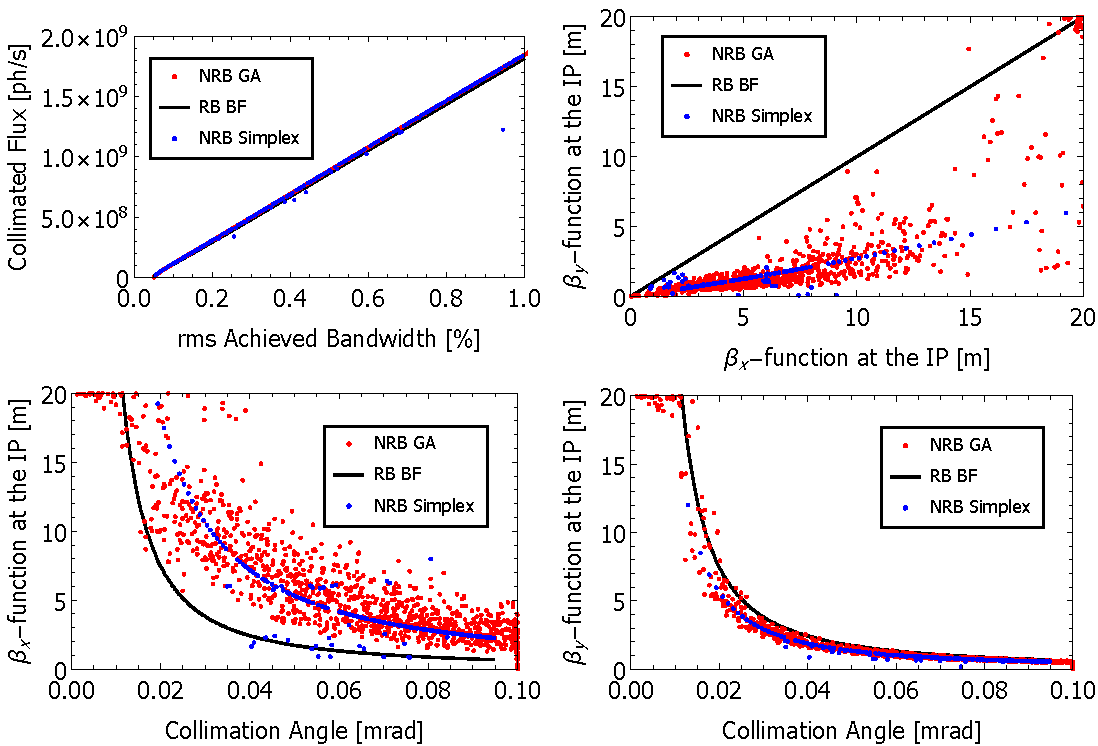
\includegraphics[width=\textwidth]{Figures/Optimisation_and_Characterisation_of_Inverse_Compton_Scattering_Sources/CaseAoptcomp.pdf}
\caption{Comparison of the three optimisation methods: RB (black), GA NRB (red) and simplex NRB (blue), trialed in high flux narrowband ICS optimisation via transverse electron bunch profile studies for the case A parameters (see Table~\ref{tab:char_opt_electron_bunch_parameters}). Top Left: Solution space ($\mathcal{F}_{\mathrm{col}}$--$\left(\Delta E_{\gamma}/E_{\gamma}\right)_{\mathrm{rms}}$) Pareto-optimal fronts. Top Right: Parameter space ($\beta_{x}^{*}$--$\beta_{y}^{*}$) variable fronts corresponding to the Pareto-optimal fronts in solution space. Bottom Left: Parameter space ($\beta_{x}^{*}$--$\theta_{\mathrm{col}}$) variable fronts corresponding to the Pareto-optimal fronts in solution space. Bottom Right: Parameter space ($\beta_{y}^{*}$--$\theta_{\mathrm{col}}$) variable fronts corresponding to the Pareto-optimal fronts in solution space.}
\label{eq:case_A_optimisation_comparison}
\end{figure}

\textcolor{blue}{**CASE A PARAMETER SPACE**}
The $\beta$-function at the IP parameter space tuning curve in Fig.~\ref{fig:case_A_optimisation_comparison} clearly shows that the non-round transverse profile solution is favoured in case A. The simplex optimisation results show good agreement with the genetic algorithm results, with the latter showing a spread of possible solutions which which is less concentrated after $\beta_{x}^{*} = 15$~\si{\meter}. The simplex optimisation shows a strongly linear relationship between the $\beta$-functions. 

The $\beta_{x}^{*}$--$\theta_{\mathrm{col}}$ parameter space plot for the case A electron bunch parameters shows a series of plots which all have the characteristic elbow shape, however the NRB GA results are stratified, though the simplex method does show good agreement with the genetic algorithm method. Some anomalous points are visible in the simplex data set which closely conform to the round transverse profile optimisation solution. The $\beta_{x}^{*}$--$\theta_{\mathrm{col}}$ tuning curve of the NRB solution appears translated, with larger $\beta_{x}^{*}$ functions for the same collimation angle. Fig.~\ref{fig:case_A_optimisation_comparison} also shows the $\beta_{y}^{*}$--$\theta_{\mathrm{col}}$ plot which again shows the characteristic elbow shape. The simplex and genetic algorithm parameter space tuning curves show good agreement, with less stratification in the $\beta_{y}^{*}$ parameter than in the $\beta$-function at the IP in the $x$ plane. The variation between the round beam and non-round beam optimisations is of a smaller magnitude than the $\beta_{x}^{*}$--$\theta_{\mathrm{col}}$ tuning curve with smaller $\beta_{y}^{*}$-functions favoured.   

\textcolor{blue}{**CASE B SOLUTION SPACE** \\ simplex fails at the narrowband end, lots of spureious points}
The collimated flux against \textit{rms} bandwidth tuning curves for each of the optimisation methods are shown in Fig.~\ref{fig:case_B_optimisation_comparison)} for a 0--2\% bandwidth range. The collimated flux--\textit{rms} bandwidth tuning curve shows that the NRB optimisation methods show generally good agreement. However, there are many anomalous local minima points within the simplex data set -- the parameter space in this case may be more complicated. At the minimum bandwidth region of the tuning curve there is also a discrepancy between the simplex and genetic algorithm methods where the GA Pareto-optimal front becomes curved and non-linear whereas the simplex method remains linear. The cause of this discrepancy is unknown but is likely to arise due to the lack of individuals in the GA simulation at the narrowband end.

\begin{figure}[!h]
\centering
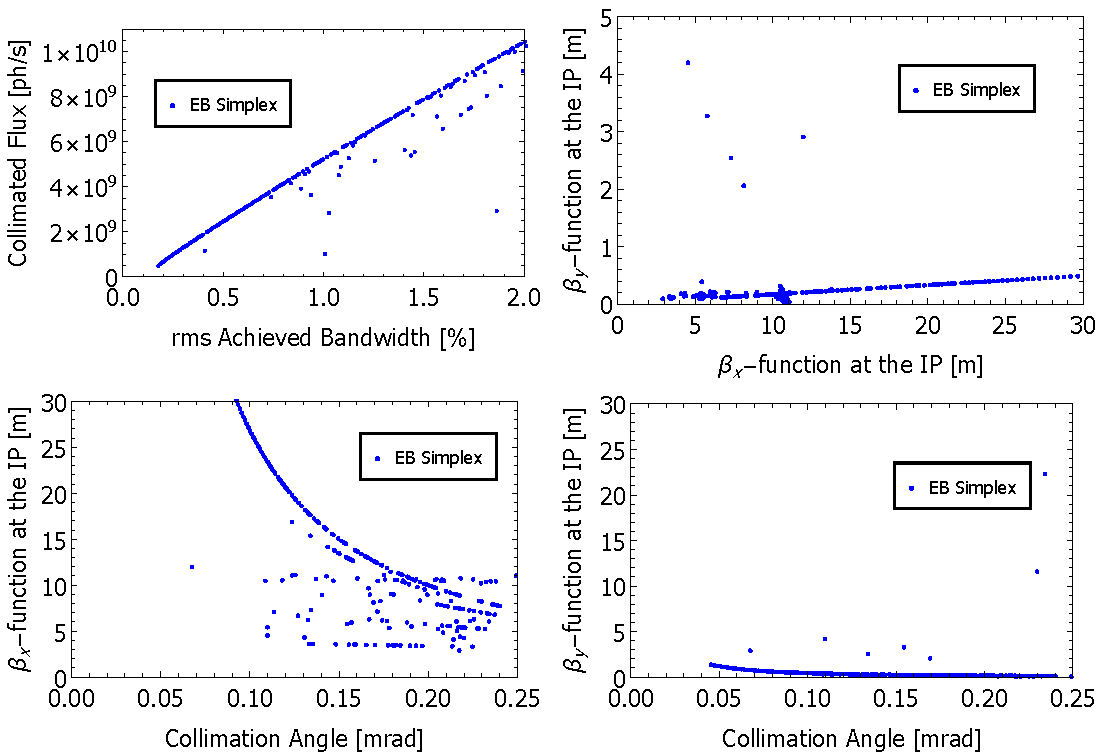
\includegraphics[width=\textwidth]{Figures/Optimisation_and_Characterisation_of_Inverse_Compton_Scattering_Sources/CaseBoptcomp.pdf}
\caption{Comparison of the two optimisation methods: Simplex NRB (blue) and GA NRB (red), trialed in high flux narrowband ICS optimisation via transverse electron bunch profile studies for the case B parameters (see Table~\ref{tab:char_opt_electron_bunch_parameters}). Top Left: Solution space ($\mathcal{F}_{\mathrm{col}}$--$\left(\Delta E_{\gamma}/E_{\gamma}\right)_{\mathrm{rms}}$) Pareto-optimal fronts. Top Right: Parameter space ($\beta_{x}^{*}$--$\beta_{y}^{*}$) variable fronts corresponding to the Pareto-optimal fronts in solution space. Bottom Left: Parameter space ($\beta_{x}^{*}$--$\theta_{\mathrm{col}}$) variable fronts corresponding to the Pareto-optimal fronts in solution space. Bottom Right: Parameter space ($\beta_{y}^{*}$--$\theta_{\mathrm{col}}$) variable fronts corresponding to the Pareto-optimal fronts in solution space.}
\label{fig:case_B_optimisation_comparison)}
\end{figure}

\textcolor{blue}{**CASE B PARAMETER SPACE**}
The $\beta$-function at the IP parameter space in Fig.~\ref{fig:case_B_optimisation_comparison)} shows that the solutions to the NRB optimisation are strongly biased toward a larger $\beta_{x}^{*}$ and smaller $\beta_{y}^{*}$. The tuning curves for the simplex and GA NRB optimisation methods agree well though there are some anomalous local minima points withing the simplex dataset and some points are clustered around $\beta_{x}^{*} = 10$~\si{\meter}.

\textcolor{blue}{**CASE C SOLUTION SPACE** \\ wait until we have simplex for this}

\begin{figure}[!h]
\centering
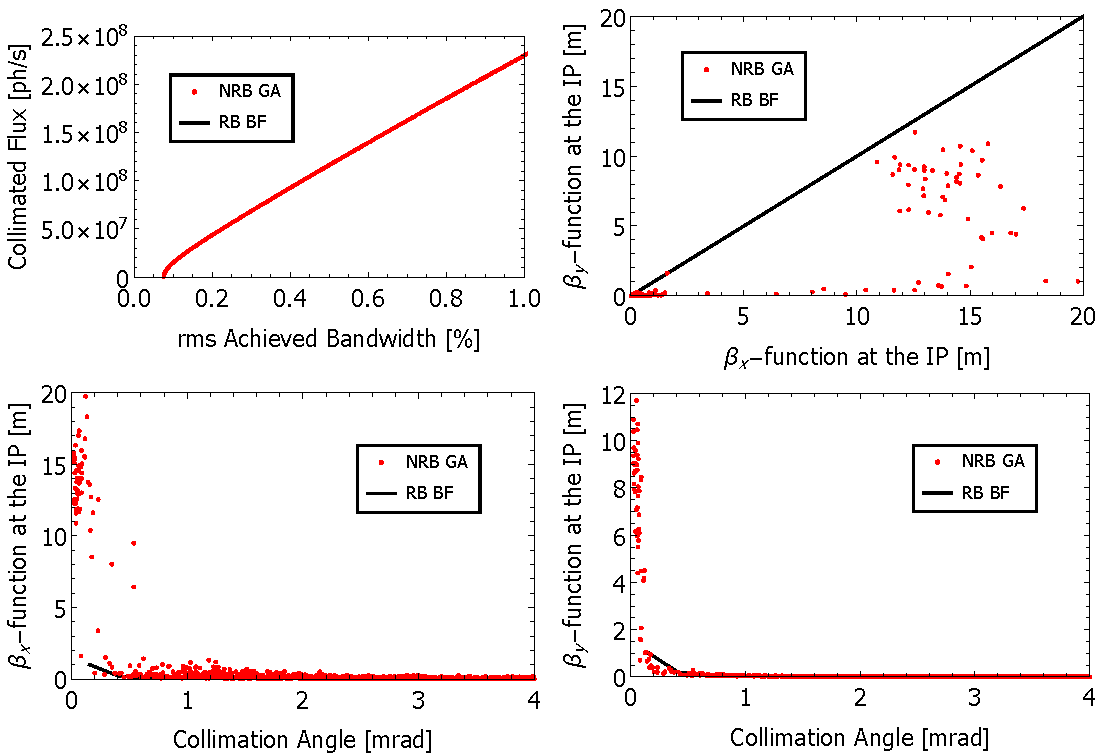
\includegraphics[width=\textwidth]{Figures/Optimisation_and_Characterisation_of_Inverse_Compton_Scattering_Sources/CaseCoptcomp.pdf}
\caption{\textcolor{blue}{**WROTE WITH SIMPLEX DISCOUNTED, NEED STATEMENT ON THIS?**}Comparison of the three optimisation methods: RB (black), GA NRB (red) and simplex NRB (blue), trialed in high flux narrowband ICS optimisation via transverse electron bunch profile studies for the case C parameters (see Table~\ref{tab:char_opt_electron_bunch_parameters}). Top Left: Solution space ($\mathcal{F}_{\mathrm{col}}$--$\left(\Delta E_{\gamma}/E_{\gamma}\right)_{\mathrm{rms}}$) Pareto-optimal fronts. Top Right: Parameter space ($\beta_{x}^{*}$--$\beta_{y}^{*}$) variable fronts corresponding to the Pareto-optimal fronts in solution space. Bottom Left: Parameter space ($\beta_{x}^{*}$--$\theta_{\mathrm{col}}$) variable fronts corresponding to the Pareto-optimal fronts in solution space. Bottom Right: Parameter space ($\beta_{y}^{*}$--$\theta_{\mathrm{col}}$) variable fronts corresponding to the Pareto-optimal fronts in solution space.}
\label{fig:case_C_optimisation_comparision}
\end{figure}

\textcolor{blue}{**CASE C PARAMETER SPACE**}

\textcolor{blue}{**SUM UP ALL OF THE METHODS**}

\section{Summary}

\end{document}